%%%%%% Run at command line, run
%%%%%% xelatex grad-sample.tex 
%%%%%% for a few times to generate the output pdf file
\documentclass[12pt,oneside,openright,a4paper]{cpe-thai-project}

\usepackage{enumitem}
\usepackage{polyglossia}
\usepackage{multirow}
\usepackage[table,xcdraw]{xcolor}
\usepackage{colortbl}
\usepackage{geometry}
\geometry{margin=1in}
\setdefaultlanguage{thai}
\setotherlanguage{english}
\newfontfamily\thaifont[Script=Thai,Scale=1.23]{TH Sarabun New}
\defaultfontfeatures{Mapping=tex-text,Scale=1.23,LetterSpace=0.0}
\setmainfont[Scale=1.23,LetterSpace=0,WordSpace=1.0,FakeStretch=1.0,Mapping=tex-text]{TH Sarabun New}
\XeTeXlinebreaklocale "th"	
\XeTeXlinebreakskip = 0pt plus 0pt
\emergencystretch=10pt

%%%%%%%%%%%%%%%%%%%%%%%%%%%%%%%%%%%%%%%%%%%%%%%%%%%%%%%%%%%%%%%%%%%
% Customize below to suit your needs 
% The ones that are optional can be left blank. 
%%%%%%%%%%%%%%%%%%%%%%%%%%%%%%%%%%%%%%%%%%%%%%%%%%%%%%%%%%%%%%%%%%%
% First line of title
\def\disstitleone{คัสตอมไอเอ (CustomAI) แพลตฟอร์มสำหรับสร้างและปรับแต่งแบบจำลองเชิงลึกจากฐานข้อมูลรูปภาพ}   
% Second line of title
\def\disstitletwo{CustomAI Platform for Deep Learning Model Creation and Customization from Image Datasets}   
% Your first name and lastname
\def\dissauthor{นายภาณุเมธ	คงสวัสดิ์เกียรติ	64070501041}   % 1st member
%%% Put other group member names here ..
\def\dissauthortwo{นายชินพรรธน์	โกปาราเมศไตรสิน	64070501061}   % 2nd member (optional)
\def\dissauthorthree{นายพัสกร	ธัญวัฒนกุล	64070501078}   % 3rd member (optional)


% The degree that you're persuing..
\def\dissdegree{Bachelor of Engineering} % Name of the degree
\def\dissdegreeabrev{B.Eng} % Abbreviation of the degree
\def\dissyear{2024}                   % Year of submission
\def\thaidissyear{2567}               % Year of submission (B.E.)

%%%%%%%%%%%%%%%%%%%%%%%%%%%%%%%%%%%%%%%%%%%%
% Your project and independent study committee..
%%%%%%%%%%%%%%%%%%%%%%%%%%%%%%%%%%%%%%%%%%%%
\def\dissadvisor{ดร.ปิยนิตย์ เวปุลานนท์}  % Advisor
%%% Leave it empty if you have no Co-advisor
\def\disscoadvisor{ดร.จาตุรนต์ หาญสมบูรณ์}  % Co-advisor
\def\disscoadvisortwo{}  % Co-advisor 2 (if any)
\def\disscoadvisorthree{}  % Co-advisor 3 (You better be building space rocket or curing cancer at this point)
\def\disscommitteetwo{Asst.Prof. Committee2, Ph.D.}  % 3rd committee member (optional)
\def\disscommitteethree{Asst.Prof. Committee3, Ph.D.}   % 4th committee member (optional) 
\def\disscommitteefour{}    % 5th committee member (optional) 

\def\worktype{Project} %%  Project or Independent study
\def\disscredit{3}   %% 3 credits or 6 credits


\def\fieldofstudy{Computer Engineering} 
\def\department{Computer Engineering} 
\def\faculty{Engineering}

\def\thaifieldofstudy{วิศวกรรมคอมพิวเตอร์} 
\def\thaidepartment{วิศวกรรมคอมพิวเตอร์} 
\def\thaifaculty{วิศวกรรมศาสตร์}
 
\def\appendixnames{Appendix} %%% Appendices or Appendix

\def\thaiworktype{ปริญญานิพนธ์} %  Project or research project % 
\def\thaidisstitleone{คัสตอมไอเอ (CustomAI) แพลตฟอร์มสำหรับสร้างและปรับแต่งแบบจำลองเชิงลึกจากฐานข้อมูลรูปภาพ}
\def\thaidisstitletwo{CustomAI Platform for Deep Learning Model Creation and Customization from Image Datasets}
\def\thaidissauthor{นายภาณุเมธ คงสวัสดิ์เกียรติ}
\def\thaidissauthortwo{นายชินพรรธน์	 โกปาราเมศไตรสิน} %Optional
\def\thaidissauthorthree{นายพัสกร ธัญวัฒนกุล} %Optional

\def\thaidissadvisor{ดร.ปิยนิตย์ เวปุลานนท์}
%% Leave this empty if you have no co-advisor
\def\thaidisscoadvisor{ดร.จาตุรนต์ หาญสมบูรณ์} %Optional
\def\thaidisscoadvisortwo{}% Co-advisor 2 (if any)
\def\thaidisscoadvisorthree{} % Co-advisor 3 (You better be building space rocket or curing cancer at this point)
\def\thaidissdegree{วิศวกรรมศาสตรบัณฑิต}

% Change the line spacing here...
\linespread{1.15}

%%%%%%%%%%%%%%%%%%%%%%%%%%%%%%%%%%%%%%%%%%%%%%%%%%%%%%%%%%%%%%%%
% End of personal customization.  Do not modify from this part 
% to \begin{document} unless you know what you are doing...
%%%%%%%%%%%%%%%%%%%%%%%%%%%%%%%%%%%%%%%%%%%%%%%%%%%%%%%%%%%%%%%%


%%%%%%%%%%%% Dissertation style %%%%%%%%%%%
%\linespread{1.6} % Double-spaced  
%%\oddsidemargin    0.5in
%%\evensidemargin   0.5in
%%%%%%%%%%%%%%%%%%%%%%%%%%%%%%%%%%%%%%%%%%%
%\renewcommand{\subfigtopskip}{10pt}
%\renewcommand{\subfigbottomskip}{-5pt} 
%\renewcommand{\subfigcapskip}{-6pt} %vertical space between caption
%                                    %and figure.
%\renewcommand{\subfigcapmargin}{0pt}

\renewcommand{\topfraction}{0.85}
\renewcommand{\textfraction}{0.1}

\newtheorem{theorem}{Theorem}
\newtheorem{lemma}{Lemma}
\newtheorem{corollary}{Corollary}

\def\QED{\mbox{\rule[0pt]{1.5ex}{1.5ex}}}
\def\proof{\noindent\hspace{2em}{\itshape Proof: }}
\def\endproof{\hspace*{\fill}~\QED\par\endtrivlist\unskip}
%\newenvironment{proof}{{\sc Proof:}}{~\hfill \blacksquare}
%% The hyperref package redefines the \appendix. This one 
%% is from the dissertation.cls
%\def\appendix#1{\iffirstappendix \appendixcover \firstappendixfalse \fi \chapter{#1}}
%\renewcommand{\arraystretch}{0.8}
%%%%%%%%%%%%%%%%%%%%%%%%%%%%%%%%%%%%%%%%%%%%%%%%%%%%%%%%%%%%%%%%
%%%%%%%%%%%%%%%%%%%%%%%%%%%%%%%%%%%%%%%%%%%%%%%%%%%%%%%%%%%%%%%%

\usepackage{ragged2e}
\begin{document}

\pdfstringdefDisableCommands{%
\let\MakeUppercase\relax
}

\begin{center}
  
\includegraphics[width=2.8cm]{logo02.jpg}
\end{center}
\vspace*{-1cm}

\maketitlepage
\makesignaturepage 

%%%%%%%%%%%%%%%%%%%%%%%%%%%%%%%%%%%%%%%%%%%%%%%%%%%%%%%%%%%%%%
%%%%%%%%%%%%%%%%%%%%%% English abstract %%%%%%%%%%%%%%%%%%%%%%%
%%%%%%%%%%%%%%%%%%%%%%%%%%%%%%%%%%%%%%%%%%%%%%%%%%%%%%%%%%%%%%
\abstract

In a multihop ad hoc network, the interference among nodes is
  reduced to maximize the throughput by using a smallest transmission
  range that still preserve the network connectivity. However, most
  existing works on transmission range control focus on the
  connectivity but lack of results on the throughput performance. This
  paper analyzes the per-node saturated throughput of an IEEE 802.11b
  multihop ad hoc network with a uniform transmission range. Compared
  to simulation, our model can accurately predict the per-node
  throughput.  The results show that the maximum achievable per-node
  throughput can be as low as 11\% of the channel capacity in a normal
  set of $\alpha$ operating parameters independent of node density. However, if
  the network connectivity is considered, the obtainable throughput
  will reduce by as many as 43\% of the maximum throughput. 

\begin{flushleft}
\begin{tabular*}{\textwidth}{@{}lp{0.8\textwidth}}
\textbf{Keywords}: & Artificial Intelligent, AI  / Image Pre-processing / Model Traininเ  / Models / Image Models / Neural Networks / Deep Learning / Data Augmentation
\end{tabular*}
\end{flushleft}
\endabstract

%%%%%%%%%%%%%%%%%%%%%%%%%%%%%%%%%%%%%%%%%%%%%%%%%%%%%%%%%%%%%%
%%%%%%%%%% Thai abstract here %%%%%%%%%%%%%%%%%%%%%%%%%%%%%%%%%
%%%%%%%%%%%%%%%%%%%%%%%%%%%%%%%%%%%%%%%%%%%%%%%%%%%%%%%%%%%%%%
% {\newfontfamily\thaifont{TH Sarabun New:script=thai}[Scale=1.3]
% \XeTeXlinebreaklocale "th_TH"	
% \thaifont
\thaiabstract

เซ็นเซอร์ เอ็กซ์เพรสรองรับคอนเซปต์สหัสวรรษเมจิก อิ่มแปร้ เฟรชชี่ ชาร์ปเช็งเม้งคลาสสิก แพตเทิร์น แอลมอนด์ เพลซว้อยก๊วน ซาร์ดีนซี้เนิร์สเซอรีอีสต์ สเตเดียมเพียบแปร้โอ้ยแคมปัส จัมโบ้ช็อตแมคเคอเรลอึ๋ม สตริง แมกกาซีนสตริงผ้าห่ม ฮัลโหล ยิม รอยัลตี้

\begin{flushleft}
\begin{tabular*}{\textwidth}{@{}lp{0.8\textwidth}}
 & \\

\textbf{คำสำคัญ}: & ปัญญาประดิษฐ์ / การประมวลผลรูปภาพเบื้องต้น / การฝึกฝนแบบจำลองปัญญาประดิษฐ์  / แบบจำลอง / แบบจำลองจากฐานข้อมูลรูปภาพ / เครือข่ายประสาทเทียม / การเรียนรู้ของเครื่องเชิงลึก / การเสริมข้อมูล
\end{tabular*}
\end{flushleft}
\endabstract

%}

%%%%%%%%%%%%%%%%%%%%%%%%%%%%%%%%%%%%%%%%%%%%%%%%%%%%%%%%%%%%
%%%%%%%%%%%%%%%%%%%%%%% Acknowledgments %%%%%%%%%%%%%%%%%%%%
%%%%%%%%%%%%%%%%%%%%%%%%%%%%%%%%%%%%%%%%%%%%%%%%%%%%%%%%%%%%
\preface
ขอบคุณอาจารย์ที่ปรึกษา กรรมการ พ่อแม่พี่น้อง และเพื่อนๆ คนที่ช่วยให้งานสำเร็จ ตามต้องการ

%%%%%%%%%%%%%%%%%%%%%%%%%%%%%%%%%%%%%%%%%%%%%%%%%%%%%%%%%%%%%
%%%%%%%%%%%%%%%% ToC, List of figures/tables %%%%%%%%%%%%%%%%
%%%%%%%%%%%%%%%%%%%%%%%%%%%%%%%%%%%%%%%%%%%%%%%%%%%%%%%%%%%%%
% The three commands below automatically generate the table 
% of content, list of tables and list of figures
\tableofcontents                    
\listoftables
\listoffigures                      

%%%%%%%%%%%%%%%%%%%%%%%%%%%%%%%%%%%%%%%%%%%%%%%%%%%%%%%%%%%%%%
%%%%%%%%%%%%%%%%%%%%% List of symbols page %%%%%%%%%%%%%%%%%%%
%%%%%%%%%%%%%%%%%%%%%%%%%%%%%%%%%%%%%%%%%%%%%%%%%%%%%%%%%%%%%%
% You have to add this manually..
\listofsymbols
\begin{flushleft}
\begin{tabular}{@{}p{0.07\textwidth}p{0.7\textwidth}p{0.1\textwidth}}
\textbf{SYMBOL}  & & \textbf{UNIT} \\[0.2cm]
$\alpha$ & Test variable\hfill & m$^2$ \\
$\lambda$ & Interarival rate\hfill &  jobs/second\\
$\mu$ & Service rate\hfill & jobs/second\\
\end{tabular}
\end{flushleft}
%%%%%%%%%%%%%%%%%%%%%%%%%%%%%%%%%%%%%%%%%%%%%%%%%%%%%%%%%%%%%%
%%%%%%%%%%%%%%%%%%%%% List of vocabs & terms %%%%%%%%%%%%%%%%%
%%%%%%%%%%%%%%%%%%%%%%%%%%%%%%%%%%%%%%%%%%%%%%%%%%%%%%%%%%%%%%
% You also have to add this manually..
\listofvocab
\begin{flushleft}
\begin{tabular}{@{}p{1in}@{=\extracolsep{0.5in}}p{0.73\textwidth}}
CRUD & Create, Read, Update, Delete  
\\
UI/UX & User experience and user interface
\\
AI & Artificial intelligent
\\
CNN & Convolutional Neural Network
\\
ERD & Entity Relations Diagram
\\
\end{tabular}
\end{flushleft}

%\setlength{\parskip}{1.2mm}

%%%%%%%%%%%%%%%%%%%%%%%%%%%%%%%%%%%%%%%%%%%%%%%%%%%%%%%%%%%%%%%
%%%%%%%%%%%%%%%%%%%%%%%% Main body %%%%%%%%%%%%%%%%%%%%%%%%%%%%
%%%%%%%%%%%%%%%%%%%%%%%%%%%%%%%%%%%%%%%%%%%%%%%%%%%%%%%%%%%%%%%


\chapter{บทนำ}

\section{ที่มาและความสำคัญ} 
	
\hspace{2em}ในปัจจุบันปัญญาประดิษฐ์ได้เข้ามามีบทบาทสำคัญในหลากหลายสาขาอาชีพมากขึ้น เนื่องจากปัญญาประดิษฐ์สามารถช่วยเพิ่มประสิทธิภาพในการทำงานบางประเภทให้รวดเร็วและแม่นยำ เช่น การวินิจฉัยทางการแพทย์ การจำแนกรูปภาพ และการตีความข้อมูลจากรูปภาพ อย่างไรก็ตาม ปัญญาประดิษฐ์แต่ละตัวถูกสร้างขึ้นเพื่อเป้าหมายที่เฉพาะเจาะจง หากนำไปใช้งานผิดจุดประสงค์จะทำให้ทำงานได้ไม่เต็มประสิทธิภาพ ตัวอย่างเช่น ปัญญาประดิษฐ์ที่พัฒนาขึ้นเพื่อจดจำวัตถุทั่วไปในรูปภาพอาจไม่สามารถตรวจจับใบหน้าได้อย่างแม่นยำ และไม่สามารถนำไปวิเคราะห์รูปภาพทางการแพทย์ได้อย่างมีประสิทธิภาพ ซึ่งหมายความว่าหากสามารถสร้างปัญญาประดิษฐ์ที่เฉพาะเจาะจงกับปัญหาได้ ปัญญาประดิษฐ์นั้นอาจมีประสิทธิภาพมากกว่าปัญญาประดิษฐ์ที่สร้างมาเพื่อแก้ไขปัญหาโดยรวม แต่กระบวนการพัฒนาแบบจำลองปัญญาประดิษฐ์เหล่านี้ยังคงเป็นเรื่องยากและต้องการความชำนาญสูง ทำให้บุคคลทั่วไปไม่สามารถสร้างแบบจำลองได้หากขาดความเข้าใจและความสามารถในการเขียนโปรแกรม 

\hspace{2em}ด้วยเหตุนี้ คณะผู้จัดทำจึงต้องการสร้างทางเลือกให้บุคคลทั่วไปสามารถเข้าถึงเทคโนโลยีปัญญาประดิษฐ์จากฐานข้อมูลรูปภาพได้ง่ายขึ้น จึงเกิดเป็นความตั้งใจในการพัฒนาแพลตฟอร์มเพื่อช่วยให้ผู้ใช้สามารถสร้างแบบจำลองปัญญาประดิษฐ์จากฐานข้อมูลรูปภาพ โดยผู้ใช้งานแพลตฟอร์มไม่จำเป็นต้องมีความรู้ด้านการเขียนโปรแกรม นอกจากนี้ผู้ใช้งานยังสามารถศึกษาและเรียนรู้เกี่ยวกับการสร้างและปรับแต่งแบบจำลองปัญญาประดิษฐ์จากฐานข้อมูลรูปภาพ สร้างความรู้และความเข้าใจในการสร้างแบบจำลองปัญญาประดิษฐ์ ทำให้ผู้ใช้สามารถพัฒนาแบบจำลองที่ตอบโจทย์ปัญหาเฉพาะของตนได้อย่างมีประสิทธิภาพสูงสุด \newline

\section{ประเภทของโครงงาน}
ต้นแบบผลิตภัณฑ์ทางการค้า

\hspace{2em}แพลตฟอร์มนี้สามารถสร้างแบบจำลองปัญญาประดิษฐ์จากฐานข้อมูลรูปภาพด้วยชุดข้อมูลที่ผู้ใช้งานต้องการ มีความยืดหยุ่นในการปรับแต่งกระบวนการประมวลผลรูปภาพและการฝึกฝนแบบจำลองปัญญาประดิษฐ์ที่หลากหลาย ซึ่งผู้ใช้ยังสามารถใช้งานแบบจำลองที่สร้างขึ้นเองบนเว็บไซต์ได้ อีกทั้งแพลตฟอร์มยังมีเนื้อหาสำหรับการศึกษาเกี่ยวกับกระบวนการสร้างและพัฒนาแบบจำลองปัญญาประดิษฐ์ เพื่อสนับสนุนการเรียนรู้และเพิ่มทักษะให้กับผู้ใช้งาน


\section{โครงงานที่นำเสนอ}
\subsection{วิธีการพัฒนาโครงงาน}
สกรัม (Scrum) ระเบียบวิธีการพัฒนาซอฟต์แวร์แบบเอจายล์ (Agile) ที่มุ่งเน้นการบริหารโครงพัฒนาซอฟต์แวร์และการวางแผนงานระยะเวลาของการพัฒนาระบบในแต่ละส่วน สกรัมเป็นระเบียบการพัฒนาซอฟต์แวร์ที่มีความยืดหยุ่นและง่ายต่อการวางแผนและติดตามงาน \cite{scrum}

\subsection{จุดประสงค์ของโครงงาน}
\vskip10pt
\begin{enumerate}
\item  เพื่อให้ผู้ใช้งานสามารถสร้างแบบจำลองปัญญาประดิษฐ์จากฐานข้อมูลรูปภาพบนแพลตฟอร์มได้
\item  เพื่อให้ผู้ใช้งานใช้แพลตฟอร์มได้โดยไม่ต้องมีความรู้ด้านการเขียนโปรแกรม
\item เพื่อให้ผู้ใช้งานสามารถปรับแต่งตัวแปรที่มีผลต่อการสร้างและใช้งานแบบจำลองได้ตามที่ต้องการ ประกอบไปด้วย ตัวแปรสำหรับการประมวลผลรูปภาพ และตัวแปรในการฝึกฝนแบบจำลอง
\item เพื่อให้ผู้ใช้งานที่ไม่มีความรู้ด้านการสร้างแบบจำลองปัญญาประดิษฐ์จากฐานข้อมูลรูปภาพ สามารถเรียนรู้เนื้อหาที่เกี่ยวข้อง และฝึกฝนทักษะบนแพลตฟอร์มที่จะพัฒนาขึ้นได้
\end{enumerate}

\subsection{ขอบเขตของโครงงาน}
\vskip10pt
\begin{enumerate}
\item พัฒนาแพลตฟอร์มในรูปแบบเว็บแอปพลิเคชัน
\item แพลตฟอร์มที่มีผู้ใช้งานหลักคือผู้ที่ต้องการสร้างแบบจำลองปัญญาประดิษฐ์จากฐานข้อมูลรูปภาพ
\item ฟังก์ชันภายในแพลตฟอร์มเป็นฟังก์ชันที่มีการพัฒนาขึ้น และนำมาใช้อย่างเเพร่หลายโดยอ้างอิงจากข้อมูลที่สืบค้นได้
\item แพลตฟอร์มสามารถทำการติดป้ายกำกับข้อมูล (Data Annotation) ให้กับชุดข้อมูลในระบบได้ทั้งรูปแบบจำแนกประเภทรูปภาพ (Classification), แบบตรวจจับวัตถุภายในรูปภาพ (Object Detection) และแบบแบ่งส่วนภาพ (Segmentation)
\item แพลตฟอร์มสามารถปรับแต่งอัตราส่วนชุดข้อมูลในการฝึกฝนแบบจำลองปัญญาประดิษฐ์ได้ (Train / Test Ratio)
\item ชนิดของรูปที่นำเข้าสู่แพลตฟอร์มจะต้องอยู่ในรูปแบบของ JPG, JPEG, PNG, WEBP, และ SVG
\item แบบจำลองที่สามารถสร้างได้บนระบบจะเป็นแบบจำลองที่เรียนรู้จากชุดข้อมูลที่มีผู้สอน (Supervised Learning) เท่านั้น
\item การเรียนรู้บนแพลตฟอร์มเป็นรูปแบบของบทเรียนเชิงโต้ตอบ (Interactive Tutorials) ที่เน้นการฝึกปฏิบัติและใช้งานเพื่อให้ผู้ใช้งานมีความรู้เบื้องต้น ไม่เน้นความเข้าใจเชิงลึก
\item เนื้อหาที่สามารถเรียนรู้ได้ในระบบจะอ้างอิงจากฟังก์ชันที่มีในแพลตฟอร์มเป็นหลัก
\item มีแบบฝึกหัดเพื่อวัดผลลัพธ์การเรียนรู้ (Learning Outcomes) จากความแม่นยำของแบบจำลองที่ถูกสร้างขึ้นผ่านการทดสอบด้วยชุดข้อมูลในแต่ละแบบฝึกหัด และการใช้ความรู้ที่ได้จากบทเรียน
\end{enumerate}

\section{เนื้อหาทางวิศวกรรมที่เป็นต้นฉบับ}
\hspace{2em}โครงงานนี้พัฒนาขึ้นจากการใช้ความรู้ในการพัฒนาเว็บไซต์ การสร้างปัญญาประดิษฐ์ การจัดการฐานข้อมูลและวิศวกรรมซอฟต์แวร์ เพื่อสร้างแพลตฟอร์มที่ผู้ใช้งานสามารถสร้างแบบจำลองปัญญาประดิษฐ์จากฐานข้อมูลรูปภาพได้โดยไม่ต้องเขียนโปรแกรม และเปิดโอกาสให้ผู้ใช้งานสามารถปรับแต่งโครงสร้างแบบจำลองและการประมวลผลรูปภาพได้มากที่สุด

\section{ตารางการดําเนินงาน}
\vskip4pt
\hspace{2em}ขั้นตอนการดําเนินงานมีดังนี้
\begin{enumerate}
\item ศึกษาข้อมูลของหัวข้อโครงงานที่ได้รับ
	\begin{enumerate}[label=\alph*.]
	\item หาข้อมูลที่เกี่ยวข้องกับโครงงานผ่านอินเทอร์เน็ตและปรึกษาอาจารย์ที่ปรึกษา
	\item ศึกษาตลาดและทดลองใช้แพลตฟอร์มที่มีความใกล้เคียงกับโครงงานเพื่อทําการเปรียบเทียบฟังก์ชันความสามารถของแต่ละเว็บไซต์
	\end{enumerate}
\item จัดทําข้อเสนอหัวข้อโครงการ (Project Idea)
\item จัดทําข้อเสนอโครงการ (Project Proposal)
\item ศึกษาเทคโนโลยีและซอฟต์แวร์ที่จะใช้
	\begin{enumerate}[label=\alph*.]
	\item เว็บไซต์ส่วนหน้า (Front-End)
	\item เว็บไซต์ส่วนหลัง (Back-End)
	\item การติดป้ายกำกับข้อมูล
	\item การประมวลผลรูปภาพเบื้องต้น
	\item การเสริมข้อมูล
	\item การฝึกฝนปัญญาประดิษฐ์สำหรับฐานข้อมูลรูปภาพ
	\end{enumerate}
\item การออกแบบระบบ
	\begin{enumerate}[label=\alph*.]
	\item ออกแบบโครงสร้างของซอฟต์แวร์และรูปแบบการใช้งาน
	\item ออกแบบฐานข้อมูลและแบบจำลองอธิบายโครงสร้างฐานข้อมูลเชิงสัมพันธ์ 
	\item (Entity Relations Diagram, ERD) เพื่อรองรับข้อมูลที่เกี่ยวข้อง
	\item ออกแบบฟังก์ชันที่สามารถใช้งานได้ในแพลตฟอร์ม
	\item ออกแบบส่วนต่อประสานกับผู้ใช้
	\item ออกแบบส่วนต่อประสานกับผู้ใช้ให้เหมาะสม ใช้งานง่าย และผู้ใช้งานสามารถเรียนรู้การใช้งานได้รวดเร็ว
	\item ออกแบบระบบการฝึกฝนแบบจำลอง
	\end{enumerate}
\item จัดทํารายงานประจําภาคการศึกษาที่ 1
\item การพัฒนาและทดสอบระบบ
	\begin{enumerate}[label=\alph*.]
	\item พัฒนาแต่ละฟีเจอร์ตามแผนที่กำหนดไว้
	\item ทดสอบหาข้อผิดพลาดของระบบและทำการแก้ไขหากตรวจพบ
	\end{enumerate}
\item ตรวจสอบระบบครั้งสุดท้าย
\item การนำระบบขึ้นสู่สาธารณะ
	\begin{enumerate}[label=\alph*.]
	\item จัดเตรียมเซิร์ฟเวอร์สำหรับการนำขึ้นสู่สาธารณะและตั้งค่าสภาพแวดล้อมในการทำงานต่าง ๆ
	\item ทำการนำระบบขึ้นโดยใช้เครื่องมือที่เหมาะสม (เช่น Docker, Kubernetes)
	\item ตรวจสอบหลังนำระบบขึ้นสำเร็จ และทำการปรับแต่งหากพบปัญหา
	\end{enumerate}
\item จัดทํารายงานประจําภาคการศึกษาที่ 2
\item นําเสนอผลงาน
\end{enumerate}

\section{แผนการดําเนินงานในภาคการศึกษาที่ 1}
\subsection{แผนการดําเนินงานเบื้องต้น}
\vskip8pt
\hspace{2em}แผนการดำเนินงานเบื้องต้นในภาคการศึกษาที่ 1 แสดงได้ดังตารางที่~\ref{tbl:method1}.
\begin{table}[h]
\caption{ตารางแสดงแผนการดำเนินงานแต่ละสัปดาห์ระหว่างเดือนสิงหาคมถึงเดือนธันวาคม 2567}\label{tbl:method1}
\begin{tabular}{|lllll|llll|llll|llll|llll|llll|}
\hline
\multicolumn{5}{|l|}{} & \multicolumn{4}{c|}{\textbf{สิงหาคม 2567}} & \multicolumn{4}{c|}{\textbf{กันยายน 2567}} & \multicolumn{4}{c|}{\textbf{ตุลาคม 2567}} & \multicolumn{4}{c|}{\textbf{พฤศจิกายน 2567}} & \multicolumn{4}{c|}{\textbf{ธันวาคม 2567}} \\ \cline{6-25} 
\multicolumn{5}{|l|}{\multirow{-2}{*}{\textbf{\begin{tabular}[c]{@{}l@{}}แผนการดำเนินงาน\\ แต่ละสัปดาห์\end{tabular}}}} & \multicolumn{1}{c|}{\textbf{1}} & \multicolumn{1}{c|}{\textbf{2}} & \multicolumn{1}{c|}{\textbf{3}} & \multicolumn{1}{c|}{\textbf{4}} & \multicolumn{1}{c|}{\textbf{1}} & \multicolumn{1}{c|}{\textbf{2}} & \multicolumn{1}{c|}{\textbf{3}} & \multicolumn{1}{c|}{\textbf{4}} & \multicolumn{1}{c|}{\textbf{1}} & \multicolumn{1}{c|}{\textbf{2}} & \multicolumn{1}{c|}{\textbf{3}} & \multicolumn{1}{c|}{\textbf{4}} & \multicolumn{1}{c|}{\textbf{1}} & \multicolumn{1}{c|}{\textbf{2}} & \multicolumn{1}{c|}{\textbf{3}} & \multicolumn{1}{c|}{\textbf{4}} & \multicolumn{1}{c|}{\textbf{1}} & \multicolumn{1}{c|}{\textbf{2}} & \multicolumn{1}{c|}{\textbf{3}} & \multicolumn{1}{c|}{\textbf{4}} \\ \hline
\multicolumn{5}{|l|}{1. ศึกษาข้อมูลของหัวข้อโครงงานที่ได้รับ} & \multicolumn{1}{l|}{\cellcolor[HTML]{C0C0C0}} & \multicolumn{1}{l|}{\cellcolor[HTML]{C0C0C0}} & \multicolumn{1}{l|}{\cellcolor[HTML]{C0C0C0}} &  & \multicolumn{1}{l|}{} & \multicolumn{1}{l|}{} & \multicolumn{1}{l|}{} &  & \multicolumn{1}{l|}{} & \multicolumn{1}{l|}{} & \multicolumn{1}{l|}{} &  & \multicolumn{1}{l|}{} & \multicolumn{1}{l|}{} & \multicolumn{1}{l|}{} &  & \multicolumn{1}{l|}{} & \multicolumn{1}{l|}{} & \multicolumn{1}{l|}{} &  \\ \hline
\multicolumn{5}{|l|}{2. จัดทําข้อเสนอหัวข้อโครงการ (Project Idea)} & \multicolumn{1}{l|}{} & \multicolumn{1}{l|}{\cellcolor[HTML]{C0C0C0}} & \multicolumn{1}{l|}{\cellcolor[HTML]{C0C0C0}} &  & \multicolumn{1}{l|}{} & \multicolumn{1}{l|}{} & \multicolumn{1}{l|}{} &  & \multicolumn{1}{l|}{} & \multicolumn{1}{l|}{} & \multicolumn{1}{l|}{} &  & \multicolumn{1}{l|}{} & \multicolumn{1}{l|}{} & \multicolumn{1}{l|}{} &  & \multicolumn{1}{l|}{} & \multicolumn{1}{l|}{} & \multicolumn{1}{l|}{} &  \\ \hline
\multicolumn{5}{|l|}{3. จัดทําข้อเสนอโครงการ (Project Proposal)} & \multicolumn{1}{l|}{} & \multicolumn{1}{l|}{} & \multicolumn{1}{l|}{} & \cellcolor[HTML]{C0C0C0}{\color[HTML]{C0C0C0} } & \multicolumn{1}{l|}{\cellcolor[HTML]{C0C0C0}{\color[HTML]{C0C0C0} }} & \multicolumn{1}{l|}{} & \multicolumn{1}{l|}{} &  & \multicolumn{1}{l|}{} & \multicolumn{1}{l|}{} & \multicolumn{1}{l|}{} &  & \multicolumn{1}{l|}{} & \multicolumn{1}{l|}{} & \multicolumn{1}{l|}{} &  & \multicolumn{1}{l|}{} & \multicolumn{1}{l|}{} & \multicolumn{1}{l|}{} &  \\ \hline
\multicolumn{5}{|l|}{4. ศึกษาเทคโนโลยีและซอฟต์แวร์ที่จะใช้} & \multicolumn{1}{l|}{} & \multicolumn{1}{l|}{} & \multicolumn{1}{l|}{} &  & \multicolumn{1}{l|}{\cellcolor[HTML]{C0C0C0}} & \multicolumn{1}{l|}{\cellcolor[HTML]{C0C0C0}} & \multicolumn{1}{l|}{\cellcolor[HTML]{C0C0C0}} & \cellcolor[HTML]{C0C0C0} & \multicolumn{1}{l|}{\cellcolor[HTML]{C0C0C0}} & \multicolumn{1}{l|}{} & \multicolumn{1}{l|}{} &  & \multicolumn{1}{l|}{} & \multicolumn{1}{l|}{} & \multicolumn{1}{l|}{} &  & \multicolumn{1}{l|}{} & \multicolumn{1}{l|}{} & \multicolumn{1}{l|}{} &  \\ \hline
\multicolumn{5}{|l|}{5. ออกแบบระบบ} & \multicolumn{1}{l|}{} & \multicolumn{1}{l|}{} & \multicolumn{1}{l|}{} &  & \multicolumn{1}{l|}{} & \multicolumn{1}{l|}{} & \multicolumn{1}{l|}{} &  & \multicolumn{1}{l|}{\cellcolor[HTML]{C0C0C0}{\color[HTML]{C0C0C0} }} & \multicolumn{1}{l|}{\cellcolor[HTML]{C0C0C0}{\color[HTML]{C0C0C0} }} & \multicolumn{1}{l|}{\cellcolor[HTML]{C0C0C0}{\color[HTML]{C0C0C0} }} & \cellcolor[HTML]{C0C0C0}{\color[HTML]{C0C0C0} } & \multicolumn{1}{l|}{} & \multicolumn{1}{l|}{} & \multicolumn{1}{l|}{} &  & \multicolumn{1}{l|}{} & \multicolumn{1}{l|}{} & \multicolumn{1}{l|}{} &  \\ \hline
\multicolumn{5}{|l|}{6. จัดทํารายงานประจําภาคการศึกษาที่ 1} & \multicolumn{1}{l|}{} & \multicolumn{1}{l|}{} & \multicolumn{1}{l|}{} &  & \multicolumn{1}{l|}{} & \multicolumn{1}{l|}{} & \multicolumn{1}{l|}{} &  & \multicolumn{1}{l|}{} & \multicolumn{1}{l|}{} & \multicolumn{1}{l|}{} & \cellcolor[HTML]{C0C0C0} & \multicolumn{1}{l|}{\cellcolor[HTML]{C0C0C0}} & \multicolumn{1}{l|}{\cellcolor[HTML]{C0C0C0}} & \multicolumn{1}{l|}{\cellcolor[HTML]{C0C0C0}} &  & \multicolumn{1}{l|}{} & \multicolumn{1}{l|}{} & \multicolumn{1}{l|}{} &  \\ \hline
\end{tabular}
\end{table}
\section{ผลการดําเนินงานในภาคการศึกษาที่ 2}
\subsection{แผนการดําเนินงานเบื้องต้น}
\vskip8pt
\hspace{2em}แผนการดำเนินงานเบื้องต้นในภาคการศึกษาที่ 2 แสดงได้ดังตารางที่~\ref{tbl:method2}.
\begin{table}[h]
\caption{ตารางแสดงแผนการดำเนินงานแต่ละสัปดาห์ระหว่างเดือนมกราคมถึงเดือนเมษายน 2568}\label{tbl:method2}
\begin{tabular}{|lllll|llll|llll|llll|llll|}
\hline
\multicolumn{5}{|l|}{} & \multicolumn{4}{c|}{\cellcolor[HTML]{FFFFFF}{\color[HTML]{000000} \textbf{มกราคม 2568}}} & \multicolumn{4}{c|}{\cellcolor[HTML]{FFFFFF}{\color[HTML]{000000} \textbf{กุมภาพันธ์ 2568}}} & \multicolumn{4}{c|}{\cellcolor[HTML]{FFFFFF}{\color[HTML]{000000} \textbf{มีนาคม 2568}}} & \multicolumn{4}{c|}{\cellcolor[HTML]{FFFFFF}{\color[HTML]{000000} \textbf{เมษายน 2568}}} \\ \cline{6-21} 
\multicolumn{5}{|l|}{\multirow{-2}{*}{\textbf{\begin{tabular}[c]{@{}l@{}}แผนการดำเนินงาน\\ แต่ละสัปดาห์\end{tabular}}}} & \multicolumn{1}{c|}{\textbf{1}} & \multicolumn{1}{c|}{\textbf{2}} & \multicolumn{1}{c|}{\textbf{3}} & \multicolumn{1}{c|}{\textbf{4}} & \multicolumn{1}{c|}{\textbf{1}} & \multicolumn{1}{c|}{\textbf{2}} & \multicolumn{1}{c|}{\textbf{3}} & \multicolumn{1}{c|}{\textbf{4}} & \multicolumn{1}{c|}{\textbf{1}} & \multicolumn{1}{c|}{\textbf{2}} & \multicolumn{1}{c|}{\textbf{3}} & \multicolumn{1}{c|}{\textbf{4}} & \multicolumn{1}{c|}{\textbf{1}} & \multicolumn{1}{c|}{\textbf{2}} & \multicolumn{1}{c|}{\textbf{3}} & \multicolumn{1}{c|}{\textbf{4}} \\ \hline
\multicolumn{5}{|l|}{1. พัฒนาและทดสอบระบบ} & \multicolumn{1}{l|}{\cellcolor[HTML]{C0C0C0}} & \multicolumn{1}{l|}{\cellcolor[HTML]{C0C0C0}} & \multicolumn{1}{l|}{\cellcolor[HTML]{C0C0C0}} & \cellcolor[HTML]{C0C0C0} & \multicolumn{1}{l|}{\cellcolor[HTML]{C0C0C0}} & \multicolumn{1}{l|}{\cellcolor[HTML]{C0C0C0}} & \multicolumn{1}{l|}{\cellcolor[HTML]{C0C0C0}} & \cellcolor[HTML]{C0C0C0} & \multicolumn{1}{l|}{\cellcolor[HTML]{C0C0C0}} & \multicolumn{1}{l|}{\cellcolor[HTML]{C0C0C0}} & \multicolumn{1}{l|}{\cellcolor[HTML]{C0C0C0}} & \cellcolor[HTML]{C0C0C0} & \multicolumn{1}{l|}{\cellcolor[HTML]{FFFFFF}} & \multicolumn{1}{l|}{\cellcolor[HTML]{FFFFFF}} & \multicolumn{1}{l|}{\cellcolor[HTML]{FFFFFF}} & \cellcolor[HTML]{FFFFFF} \\ \hline
\multicolumn{5}{|l|}{2. ตรวจสอบระบบครั้งสุดท้าย} & \multicolumn{1}{l|}{\cellcolor[HTML]{FFFFFF}} & \multicolumn{1}{l|}{\cellcolor[HTML]{FFFFFF}} & \multicolumn{1}{l|}{\cellcolor[HTML]{FFFFFF}} & \cellcolor[HTML]{FFFFFF} & \multicolumn{1}{l|}{\cellcolor[HTML]{FFFFFF}} & \multicolumn{1}{l|}{\cellcolor[HTML]{FFFFFF}} & \multicolumn{1}{l|}{\cellcolor[HTML]{FFFFFF}} & \cellcolor[HTML]{FFFFFF} & \multicolumn{1}{l|}{\cellcolor[HTML]{FFFFFF}} & \multicolumn{1}{l|}{\cellcolor[HTML]{FFFFFF}} & \multicolumn{1}{l|}{\cellcolor[HTML]{C0C0C0}} & \cellcolor[HTML]{C0C0C0} & \multicolumn{1}{l|}{\cellcolor[HTML]{C0C0C0}} & \multicolumn{1}{l|}{\cellcolor[HTML]{FFFFFF}} & \multicolumn{1}{l|}{\cellcolor[HTML]{FFFFFF}} & \cellcolor[HTML]{FFFFFF} \\ \hline
\multicolumn{5}{|l|}{3. นำระบบขึ้นสู่สาธารณะ} & \multicolumn{1}{l|}{\cellcolor[HTML]{FFFFFF}} & \multicolumn{1}{l|}{\cellcolor[HTML]{FFFFFF}} & \multicolumn{1}{l|}{\cellcolor[HTML]{FFFFFF}} & \cellcolor[HTML]{FFFFFF}{\color[HTML]{C0C0C0} } & \multicolumn{1}{l|}{\cellcolor[HTML]{FFFFFF}{\color[HTML]{C0C0C0} }} & \multicolumn{1}{l|}{\cellcolor[HTML]{FFFFFF}} & \multicolumn{1}{l|}{\cellcolor[HTML]{FFFFFF}} & \cellcolor[HTML]{FFFFFF} & \multicolumn{1}{l|}{\cellcolor[HTML]{FFFFFF}} & \multicolumn{1}{l|}{\cellcolor[HTML]{FFFFFF}} & \multicolumn{1}{l|}{\cellcolor[HTML]{C0C0C0}} & \cellcolor[HTML]{C0C0C0} & \multicolumn{1}{l|}{\cellcolor[HTML]{FFFFFF}} & \multicolumn{1}{l|}{\cellcolor[HTML]{FFFFFF}} & \multicolumn{1}{l|}{\cellcolor[HTML]{FFFFFF}} & \cellcolor[HTML]{FFFFFF} \\ \hline
\multicolumn{5}{|l|}{4. จัดทํารายงานประจําภาคการศึกษาที่ 2} & \multicolumn{1}{l|}{\cellcolor[HTML]{FFFFFF}} & \multicolumn{1}{l|}{\cellcolor[HTML]{FFFFFF}} & \multicolumn{1}{l|}{\cellcolor[HTML]{FFFFFF}} & \cellcolor[HTML]{FFFFFF} & \multicolumn{1}{l|}{\cellcolor[HTML]{FFFFFF}} & \multicolumn{1}{l|}{\cellcolor[HTML]{FFFFFF}} & \multicolumn{1}{l|}{\cellcolor[HTML]{FFFFFF}} & \cellcolor[HTML]{FFFFFF} & \multicolumn{1}{l|}{\cellcolor[HTML]{FFFFFF}} & \multicolumn{1}{l|}{\cellcolor[HTML]{FFFFFF}} & \multicolumn{1}{l|}{\cellcolor[HTML]{FFFFFF}} & \cellcolor[HTML]{FFFFFF} & \multicolumn{1}{l|}{\cellcolor[HTML]{C0C0C0}} & \multicolumn{1}{l|}{\cellcolor[HTML]{C0C0C0}} & \multicolumn{1}{l|}{\cellcolor[HTML]{C0C0C0}} & \cellcolor[HTML]{FFFFFF} \\ \hline
\multicolumn{5}{|l|}{5. นําเสนอผลงาน} & \multicolumn{1}{l|}{\cellcolor[HTML]{FFFFFF}} & \multicolumn{1}{l|}{\cellcolor[HTML]{FFFFFF}} & \multicolumn{1}{l|}{\cellcolor[HTML]{FFFFFF}} & \cellcolor[HTML]{FFFFFF} & \multicolumn{1}{l|}{\cellcolor[HTML]{FFFFFF}} & \multicolumn{1}{l|}{\cellcolor[HTML]{FFFFFF}} & \multicolumn{1}{l|}{\cellcolor[HTML]{FFFFFF}} & \cellcolor[HTML]{FFFFFF} & \multicolumn{1}{l|}{\cellcolor[HTML]{FFFFFF}{\color[HTML]{C0C0C0} }} & \multicolumn{1}{l|}{\cellcolor[HTML]{FFFFFF}{\color[HTML]{C0C0C0} }} & \multicolumn{1}{l|}{\cellcolor[HTML]{FFFFFF}{\color[HTML]{C0C0C0} }} & \cellcolor[HTML]{FFFFFF}{\color[HTML]{C0C0C0} } & \multicolumn{1}{l|}{\cellcolor[HTML]{FFFFFF}} & \multicolumn{1}{l|}{\cellcolor[HTML]{FFFFFF}} & \multicolumn{1}{l|}{\cellcolor[HTML]{FFFFFF}} & \cellcolor[HTML]{C0C0C0} \\ \hline
\end{tabular}
\end{table}
\subsection{แผนการดําเนินงานเชิงลึก}
\hspace{2em}แผนการดำเนินงานอย่างละเอียดในภาคเรียนที่ 2 โดยจะประกอบไปด้วยทั้งหมด 4 ตารางได้แก่
\begin{enumerate}
\item ตารางที่~\ref{tbl:method3}. ฝั่งเว็บไซต์ส่วนหลังปัญญาประดิษฐ์
	\begin{table}[h]
	\caption{ตารางแสดงแผนการดำเนินการฝั่งเว็บไซต์ส่วนหลังปัญญาประดิษฐ์แต่ละสัปดาห์ระหว่างเดือนมกราคมถึงเดือนเมษายน 2568}\label{tbl:method3}
	\begin{tabular}{|lllll|llll|llll|llll|llll|}
	\hline
	\multicolumn{5}{|l|}{} & \multicolumn{4}{c|}{\cellcolor[HTML]{FFFFFF}{\color[HTML]{000000} \textbf{มกราคม 2568}}} & \multicolumn{4}{c|}{\cellcolor[HTML]{FFFFFF}{\color[HTML]{000000} \textbf{กุมภาพันธ์ 2568}}} & \multicolumn{4}{c|}{\cellcolor[HTML]{FFFFFF}{\color[HTML]{000000} \textbf{มีนาคม 2568}}} & \multicolumn{4}{c|}{\cellcolor[HTML]{FFFFFF}{\color[HTML]{000000} \textbf{เมษายน 2568}}} \\ \cline{6-21} 
	\multicolumn{5}{|c|}{\multirow{-2}{*}{\textbf{\begin{tabular}[c]{@{}c@{}}แผนการดำเนินงาน\\ แต่ละสัปดาห์\end{tabular}}}} & \multicolumn{1}{c|}{\textbf{1}} & \multicolumn{1}{c|}{\textbf{2}} & \multicolumn{1}{c|}{\textbf{3}} & \multicolumn{1}{c|}{\textbf{4}} & \multicolumn{1}{c|}{\textbf{1}} & \multicolumn{1}{c|}{\textbf{2}} & \multicolumn{1}{c|}{\textbf{3}} & \multicolumn{1}{c|}{\textbf{4}} & \multicolumn{1}{c|}{\textbf{1}} & \multicolumn{1}{c|}{\textbf{2}} & \multicolumn{1}{c|}{\textbf{3}} & \multicolumn{1}{c|}{\textbf{4}} & \multicolumn{1}{c|}{\textbf{1}} & \multicolumn{1}{c|}{\textbf{2}} & \multicolumn{1}{c|}{\textbf{3}} & \multicolumn{1}{c|}{\textbf{4}} \\ \hline
	\rowcolor[HTML]{FFFFFF} 
	\multicolumn{5}{|l|}{\cellcolor[HTML]{FFFFFF}1. ระบบจัดการชุดข้อมูล} & \multicolumn{1}{l|}{\cellcolor[HTML]{C0C0C0}} & \multicolumn{1}{l|}{\cellcolor[HTML]{FFFFFF}} & \multicolumn{1}{l|}{\cellcolor[HTML]{FFFFFF}} &  & \multicolumn{1}{l|}{\cellcolor[HTML]{FFFFFF}} & \multicolumn{1}{l|}{\cellcolor[HTML]{FFFFFF}} & \multicolumn{1}{l|}{\cellcolor[HTML]{FFFFFF}} &  & \multicolumn{1}{l|}{\cellcolor[HTML]{FFFFFF}} & \multicolumn{1}{l|}{\cellcolor[HTML]{FFFFFF}} & \multicolumn{1}{l|}{\cellcolor[HTML]{FFFFFF}} &  & \multicolumn{1}{l|}{\cellcolor[HTML]{FFFFFF}} & \multicolumn{1}{l|}{\cellcolor[HTML]{FFFFFF}} & \multicolumn{1}{l|}{\cellcolor[HTML]{FFFFFF}} &  \\ \hline
	\rowcolor[HTML]{FFFFFF} 
	\multicolumn{5}{|l|}{\cellcolor[HTML]{FFFFFF}2. ระบบการประมวลผลรูปภาพเบื้องต้น} & \multicolumn{1}{l|}{\cellcolor[HTML]{FFFFFF}} & \multicolumn{1}{l|}{\cellcolor[HTML]{C0C0C0}} & \multicolumn{1}{l|}{\cellcolor[HTML]{C0C0C0}} &  & \multicolumn{1}{l|}{\cellcolor[HTML]{FFFFFF}} & \multicolumn{1}{l|}{\cellcolor[HTML]{FFFFFF}} & \multicolumn{1}{l|}{\cellcolor[HTML]{FFFFFF}} &  & \multicolumn{1}{l|}{\cellcolor[HTML]{FFFFFF}} & \multicolumn{1}{l|}{\cellcolor[HTML]{FFFFFF}} & \multicolumn{1}{l|}{\cellcolor[HTML]{FFFFFF}} &  & \multicolumn{1}{l|}{\cellcolor[HTML]{FFFFFF}} & \multicolumn{1}{l|}{\cellcolor[HTML]{FFFFFF}} & \multicolumn{1}{l|}{\cellcolor[HTML]{FFFFFF}} &  \\ \hline
	\rowcolor[HTML]{FFFFFF} 
	\multicolumn{5}{|l|}{\cellcolor[HTML]{FFFFFF}3. ระบบสกัดคุณลักษณะและการเลือกคุณลักษณะ} & \multicolumn{1}{l|}{\cellcolor[HTML]{FFFFFF}} & \multicolumn{1}{l|}{\cellcolor[HTML]{FFFFFF}} & \multicolumn{1}{l|}{\cellcolor[HTML]{FFFFFF}} & \cellcolor[HTML]{C0C0C0}{\color[HTML]{C0C0C0} } & \multicolumn{1}{l|}{\cellcolor[HTML]{FFFFFF}{\color[HTML]{C0C0C0} }} & \multicolumn{1}{l|}{\cellcolor[HTML]{FFFFFF}} & \multicolumn{1}{l|}{\cellcolor[HTML]{FFFFFF}} &  & \multicolumn{1}{l|}{\cellcolor[HTML]{FFFFFF}} & \multicolumn{1}{l|}{\cellcolor[HTML]{FFFFFF}} & \multicolumn{1}{l|}{\cellcolor[HTML]{FFFFFF}} &  & \multicolumn{1}{l|}{\cellcolor[HTML]{FFFFFF}} & \multicolumn{1}{l|}{\cellcolor[HTML]{FFFFFF}} & \multicolumn{1}{l|}{\cellcolor[HTML]{FFFFFF}} &  \\ \hline
	\rowcolor[HTML]{FFFFFF} 
	\multicolumn{5}{|l|}{\cellcolor[HTML]{FFFFFF}4. ระบบเสริมข้อมูล} & \multicolumn{1}{l|}{\cellcolor[HTML]{FFFFFF}} & \multicolumn{1}{l|}{\cellcolor[HTML]{FFFFFF}} & \multicolumn{1}{l|}{\cellcolor[HTML]{FFFFFF}} &  & \multicolumn{1}{l|}{\cellcolor[HTML]{C0C0C0}} & \multicolumn{1}{l|}{\cellcolor[HTML]{C0C0C0}} & \multicolumn{1}{l|}{\cellcolor[HTML]{FFFFFF}} &  & \multicolumn{1}{l|}{\cellcolor[HTML]{FFFFFF}} & \multicolumn{1}{l|}{\cellcolor[HTML]{FFFFFF}} & \multicolumn{1}{l|}{\cellcolor[HTML]{FFFFFF}} &  & \multicolumn{1}{l|}{\cellcolor[HTML]{FFFFFF}} & \multicolumn{1}{l|}{\cellcolor[HTML]{FFFFFF}} & \multicolumn{1}{l|}{\cellcolor[HTML]{FFFFFF}} &  \\ \hline
	\rowcolor[HTML]{FFFFFF} 
	\multicolumn{5}{|l|}{\cellcolor[HTML]{FFFFFF}5. ระบบสร้างแบบจำลองปัญญาประดิษฐ์} & \multicolumn{1}{l|}{\cellcolor[HTML]{FFFFFF}} & \multicolumn{1}{l|}{\cellcolor[HTML]{FFFFFF}} & \multicolumn{1}{l|}{\cellcolor[HTML]{FFFFFF}} &  & \multicolumn{1}{l|}{\cellcolor[HTML]{FFFFFF}} & \multicolumn{1}{l|}{\cellcolor[HTML]{FFFFFF}} & \multicolumn{1}{l|}{\cellcolor[HTML]{C0C0C0}} & \cellcolor[HTML]{C0C0C0} & \multicolumn{1}{l|}{\cellcolor[HTML]{FFFFFF}{\color[HTML]{C0C0C0} }} & \multicolumn{1}{l|}{\cellcolor[HTML]{FFFFFF}{\color[HTML]{C0C0C0} }} & \multicolumn{1}{l|}{\cellcolor[HTML]{FFFFFF}{\color[HTML]{C0C0C0} }} & {\color[HTML]{C0C0C0} } & \multicolumn{1}{l|}{\cellcolor[HTML]{FFFFFF}} & \multicolumn{1}{l|}{\cellcolor[HTML]{FFFFFF}} & \multicolumn{1}{l|}{\cellcolor[HTML]{FFFFFF}} &  \\ \hline
	\multicolumn{5}{|l|}{\cellcolor[HTML]{FFFFFF}6. ระบบฝึกฝนแบบจำลอง} & \multicolumn{1}{l|}{} & \multicolumn{1}{l|}{} & \multicolumn{1}{l|}{} &  & \multicolumn{1}{l|}{} & \multicolumn{1}{l|}{} & \multicolumn{1}{l|}{} &  & \multicolumn{1}{l|}{\cellcolor[HTML]{C0C0C0}} & \multicolumn{1}{l|}{\cellcolor[HTML]{C0C0C0}} & \multicolumn{1}{l|}{} &  & \multicolumn{1}{l|}{} & \multicolumn{1}{l|}{} & \multicolumn{1}{l|}{} &  \\ \hline
	\multicolumn{5}{|l|}{\cellcolor[HTML]{FFFFFF}7. ระบบวัดผลแบบจำลอง} & \multicolumn{1}{l|}{} & \multicolumn{1}{l|}{} & \multicolumn{1}{l|}{} &  & \multicolumn{1}{l|}{} & \multicolumn{1}{l|}{} & \multicolumn{1}{l|}{} &  & \multicolumn{1}{l|}{} & \multicolumn{1}{l|}{} & \multicolumn{1}{l|}{\cellcolor[HTML]{C0C0C0}} &  & \multicolumn{1}{l|}{} & \multicolumn{1}{l|}{} & \multicolumn{1}{l|}{} &  \\ \hline
	\multicolumn{5}{|l|}{\cellcolor[HTML]{FFFFFF}8. ระบบใช้งานแบบจำลองปัญญาประดิษฐ์} & \multicolumn{1}{l|}{} & \multicolumn{1}{l|}{} & \multicolumn{1}{l|}{} &  & \multicolumn{1}{l|}{} & \multicolumn{1}{l|}{} & \multicolumn{1}{l|}{} &  & \multicolumn{1}{l|}{} & \multicolumn{1}{l|}{} & \multicolumn{1}{l|}{} & \cellcolor[HTML]{C0C0C0} & \multicolumn{1}{l|}{} & \multicolumn{1}{l|}{} & \multicolumn{1}{l|}{} &  \\ \hline
	\end{tabular}
	\end{table}
\item ฝั่งเว็บไซต์ส่วนหลัง (Backend - Web Service) มีแผนการดำเนินงานดังตารางที่~\ref{tbl:method4}.
\begin{table}[h]
\caption{ตารางแสดงแผนการดำเนินการฝั่งเว็บไซต์ส่วนหลังแต่ละสัปดาห์ระหว่างเดือนมกราคมถึงเดือนเมษายน 2568}\label{tbl:method4}
\begin{tabular}{|lllll|llll|llll|llll|llll|}
\hline
\multicolumn{5}{|c|}{} & \multicolumn{4}{c|}{\cellcolor[HTML]{FFFFFF}{\color[HTML]{000000} \textbf{มกราคม 2568}}} & \multicolumn{4}{c|}{\cellcolor[HTML]{FFFFFF}{\color[HTML]{000000} \textbf{กุมภาพันธ์ 2568}}} & \multicolumn{4}{c|}{\cellcolor[HTML]{FFFFFF}{\color[HTML]{000000} \textbf{มีนาคม 2568}}} & \multicolumn{4}{c|}{\cellcolor[HTML]{FFFFFF}{\color[HTML]{000000} \textbf{เมษายน 2568}}} \\ \cline{6-21} 
\multicolumn{5}{|c|}{\multirow{-2}{*}{\textbf{\begin{tabular}[c]{@{}c@{}}แผนการดำเนินงาน\\ แต่ละสัปดาห์\end{tabular}}}} & \multicolumn{1}{c|}{\textbf{1}} & \multicolumn{1}{c|}{\textbf{2}} & \multicolumn{1}{c|}{\textbf{3}} & \multicolumn{1}{c|}{\textbf{4}} & \multicolumn{1}{c|}{\textbf{1}} & \multicolumn{1}{c|}{\textbf{2}} & \multicolumn{1}{c|}{\textbf{3}} & \multicolumn{1}{c|}{\textbf{4}} & \multicolumn{1}{c|}{\textbf{1}} & \multicolumn{1}{c|}{\textbf{2}} & \multicolumn{1}{c|}{\textbf{3}} & \multicolumn{1}{c|}{\textbf{4}} & \multicolumn{1}{c|}{\textbf{1}} & \multicolumn{1}{c|}{\textbf{2}} & \multicolumn{1}{c|}{\textbf{3}} & \multicolumn{1}{c|}{\textbf{4}} \\ \hline
\rowcolor[HTML]{FFFFFF} 
\multicolumn{5}{|l|}{\cellcolor[HTML]{FFFFFF}1. จัดเตรียมฐานข้อมูลทั้งหมด} & \multicolumn{1}{l|}{\cellcolor[HTML]{C0C0C0}} & \multicolumn{1}{l|}{\cellcolor[HTML]{FFFFFF}} & \multicolumn{1}{l|}{\cellcolor[HTML]{FFFFFF}} &  & \multicolumn{1}{l|}{\cellcolor[HTML]{FFFFFF}} & \multicolumn{1}{l|}{\cellcolor[HTML]{FFFFFF}} & \multicolumn{1}{l|}{\cellcolor[HTML]{FFFFFF}} &  & \multicolumn{1}{l|}{\cellcolor[HTML]{FFFFFF}} & \multicolumn{1}{l|}{\cellcolor[HTML]{FFFFFF}} & \multicolumn{1}{l|}{\cellcolor[HTML]{FFFFFF}} &  & \multicolumn{1}{l|}{\cellcolor[HTML]{FFFFFF}} & \multicolumn{1}{l|}{\cellcolor[HTML]{FFFFFF}} & \multicolumn{1}{l|}{\cellcolor[HTML]{FFFFFF}} &  \\ \hline
\rowcolor[HTML]{FFFFFF} 
\multicolumn{5}{|l|}{\cellcolor[HTML]{FFFFFF}2. ระบบยืนยันตัวตน} & \multicolumn{1}{l|}{\cellcolor[HTML]{C0C0C0}} & \multicolumn{1}{l|}{\cellcolor[HTML]{FFFFFF}} & \multicolumn{1}{l|}{\cellcolor[HTML]{FFFFFF}} &  & \multicolumn{1}{l|}{\cellcolor[HTML]{FFFFFF}} & \multicolumn{1}{l|}{\cellcolor[HTML]{FFFFFF}} & \multicolumn{1}{l|}{\cellcolor[HTML]{FFFFFF}} &  & \multicolumn{1}{l|}{\cellcolor[HTML]{FFFFFF}} & \multicolumn{1}{l|}{\cellcolor[HTML]{FFFFFF}} & \multicolumn{1}{l|}{\cellcolor[HTML]{FFFFFF}} &  & \multicolumn{1}{l|}{\cellcolor[HTML]{FFFFFF}} & \multicolumn{1}{l|}{\cellcolor[HTML]{FFFFFF}} & \multicolumn{1}{l|}{\cellcolor[HTML]{FFFFFF}} &  \\ \hline
\rowcolor[HTML]{FFFFFF} 
\multicolumn{5}{|l|}{\cellcolor[HTML]{FFFFFF}3. ระบบอัปโหลดไฟล์} & \multicolumn{1}{l|}{\cellcolor[HTML]{FFFFFF}} & \multicolumn{1}{l|}{\cellcolor[HTML]{C0C0C0}} & \multicolumn{1}{l|}{\cellcolor[HTML]{FFFFFF}} & {\color[HTML]{C0C0C0} } & \multicolumn{1}{l|}{\cellcolor[HTML]{FFFFFF}{\color[HTML]{C0C0C0} }} & \multicolumn{1}{l|}{\cellcolor[HTML]{FFFFFF}} & \multicolumn{1}{l|}{\cellcolor[HTML]{FFFFFF}} &  & \multicolumn{1}{l|}{\cellcolor[HTML]{FFFFFF}} & \multicolumn{1}{l|}{\cellcolor[HTML]{FFFFFF}} & \multicolumn{1}{l|}{\cellcolor[HTML]{FFFFFF}} &  & \multicolumn{1}{l|}{\cellcolor[HTML]{FFFFFF}} & \multicolumn{1}{l|}{\cellcolor[HTML]{FFFFFF}} & \multicolumn{1}{l|}{\cellcolor[HTML]{FFFFFF}} &  \\ \hline
\rowcolor[HTML]{FFFFFF} 
\multicolumn{5}{|l|}{\cellcolor[HTML]{FFFFFF}4. ระบบอัปโหลดรูปภาพ} & \multicolumn{1}{l|}{\cellcolor[HTML]{FFFFFF}} & \multicolumn{1}{l|}{\cellcolor[HTML]{C0C0C0}} & \multicolumn{1}{l|}{\cellcolor[HTML]{FFFFFF}} &  & \multicolumn{1}{l|}{\cellcolor[HTML]{FFFFFF}} & \multicolumn{1}{l|}{\cellcolor[HTML]{FFFFFF}} & \multicolumn{1}{l|}{\cellcolor[HTML]{FFFFFF}} &  & \multicolumn{1}{l|}{\cellcolor[HTML]{FFFFFF}} & \multicolumn{1}{l|}{\cellcolor[HTML]{FFFFFF}} & \multicolumn{1}{l|}{\cellcolor[HTML]{FFFFFF}} &  & \multicolumn{1}{l|}{\cellcolor[HTML]{FFFFFF}} & \multicolumn{1}{l|}{\cellcolor[HTML]{FFFFFF}} & \multicolumn{1}{l|}{\cellcolor[HTML]{FFFFFF}} &  \\ \hline
\rowcolor[HTML]{FFFFFF} 
\multicolumn{5}{|l|}{\cellcolor[HTML]{FFFFFF}5. ระบบอัปโหลดชุดข้อมูล} & \multicolumn{1}{l|}{\cellcolor[HTML]{FFFFFF}} & \multicolumn{1}{l|}{\cellcolor[HTML]{FFFFFF}} & \multicolumn{1}{l|}{\cellcolor[HTML]{C0C0C0}} &  & \multicolumn{1}{l|}{\cellcolor[HTML]{FFFFFF}} & \multicolumn{1}{l|}{\cellcolor[HTML]{FFFFFF}} & \multicolumn{1}{l|}{\cellcolor[HTML]{FFFFFF}} &  & \multicolumn{1}{l|}{\cellcolor[HTML]{FFFFFF}{\color[HTML]{C0C0C0} }} & \multicolumn{1}{l|}{\cellcolor[HTML]{FFFFFF}{\color[HTML]{C0C0C0} }} & \multicolumn{1}{l|}{\cellcolor[HTML]{FFFFFF}{\color[HTML]{C0C0C0} }} & {\color[HTML]{C0C0C0} } & \multicolumn{1}{l|}{\cellcolor[HTML]{FFFFFF}} & \multicolumn{1}{l|}{\cellcolor[HTML]{FFFFFF}} & \multicolumn{1}{l|}{\cellcolor[HTML]{FFFFFF}} &  \\ \hline
\multicolumn{5}{|l|}{\cellcolor[HTML]{FFFFFF}6. CRUD ข้อมูลระบบเสริมข้อมูล} & \multicolumn{1}{l|}{\cellcolor[HTML]{FFFFFF}} & \multicolumn{1}{l|}{\cellcolor[HTML]{FFFFFF}} & \multicolumn{1}{l|}{\cellcolor[HTML]{C0C0C0}} & \cellcolor[HTML]{FFFFFF} & \multicolumn{1}{l|}{\cellcolor[HTML]{FFFFFF}} & \multicolumn{1}{l|}{\cellcolor[HTML]{FFFFFF}} & \multicolumn{1}{l|}{\cellcolor[HTML]{FFFFFF}} & \cellcolor[HTML]{FFFFFF} & \multicolumn{1}{l|}{\cellcolor[HTML]{FFFFFF}} & \multicolumn{1}{l|}{\cellcolor[HTML]{FFFFFF}} & \multicolumn{1}{l|}{\cellcolor[HTML]{FFFFFF}} & \cellcolor[HTML]{FFFFFF} & \multicolumn{1}{l|}{} & \multicolumn{1}{l|}{} & \multicolumn{1}{l|}{} &  \\ \hline
\multicolumn{5}{|l|}{\cellcolor[HTML]{FFFFFF}7. CRUD ข้อมูลระบบสร้างแบบจำลอง} & \multicolumn{1}{l|}{\cellcolor[HTML]{FFFFFF}} & \multicolumn{1}{l|}{\cellcolor[HTML]{FFFFFF}} & \multicolumn{1}{l|}{\cellcolor[HTML]{C0C0C0}} & \cellcolor[HTML]{C0C0C0} & \multicolumn{1}{l|}{\cellcolor[HTML]{FFFFFF}} & \multicolumn{1}{l|}{\cellcolor[HTML]{FFFFFF}} & \multicolumn{1}{l|}{\cellcolor[HTML]{FFFFFF}} & \cellcolor[HTML]{FFFFFF} & \multicolumn{1}{l|}{\cellcolor[HTML]{FFFFFF}} & \multicolumn{1}{l|}{\cellcolor[HTML]{FFFFFF}} & \multicolumn{1}{l|}{\cellcolor[HTML]{FFFFFF}} & \cellcolor[HTML]{FFFFFF} & \multicolumn{1}{l|}{} & \multicolumn{1}{l|}{} & \multicolumn{1}{l|}{} &  \\ \hline
\multicolumn{5}{|l|}{\cellcolor[HTML]{FFFFFF}8. CRUD ข้อมูลฝึกฝนแบบจำลอง} & \multicolumn{1}{l|}{\cellcolor[HTML]{FFFFFF}} & \multicolumn{1}{l|}{\cellcolor[HTML]{FFFFFF}} & \multicolumn{1}{l|}{\cellcolor[HTML]{FFFFFF}} & \cellcolor[HTML]{C0C0C0} & \multicolumn{1}{l|}{\cellcolor[HTML]{C0C0C0}} & \multicolumn{1}{l|}{\cellcolor[HTML]{FFFFFF}} & \multicolumn{1}{l|}{\cellcolor[HTML]{FFFFFF}} & \cellcolor[HTML]{FFFFFF} & \multicolumn{1}{l|}{\cellcolor[HTML]{FFFFFF}} & \multicolumn{1}{l|}{\cellcolor[HTML]{FFFFFF}} & \multicolumn{1}{l|}{\cellcolor[HTML]{FFFFFF}} & \cellcolor[HTML]{FFFFFF} & \multicolumn{1}{l|}{} & \multicolumn{1}{l|}{} & \multicolumn{1}{l|}{} &  \\ \hline
\multicolumn{5}{|l|}{\cellcolor[HTML]{FFFFFF}9. CRUD ข้อมูลผลการฝึกฝนแบบจำลอง} & \multicolumn{1}{l|}{} & \multicolumn{1}{l|}{} & \multicolumn{1}{l|}{} &  & \multicolumn{1}{l|}{\cellcolor[HTML]{C0C0C0}} & \multicolumn{1}{l|}{\cellcolor[HTML]{C0C0C0}} & \multicolumn{1}{l|}{} &  & \multicolumn{1}{l|}{} & \multicolumn{1}{l|}{} & \multicolumn{1}{l|}{} &  & \multicolumn{1}{l|}{} & \multicolumn{1}{l|}{} & \multicolumn{1}{l|}{} &  \\ \hline
\multicolumn{5}{|l|}{\cellcolor[HTML]{FFFFFF}10. CRUD การเรียนรู้ - เรียนรู้} & \multicolumn{1}{l|}{} & \multicolumn{1}{l|}{} & \multicolumn{1}{l|}{} &  & \multicolumn{1}{l|}{} & \multicolumn{1}{l|}{} & \multicolumn{1}{l|}{\cellcolor[HTML]{C0C0C0}} &  & \multicolumn{1}{l|}{} & \multicolumn{1}{l|}{} & \multicolumn{1}{l|}{} &  & \multicolumn{1}{l|}{} & \multicolumn{1}{l|}{} & \multicolumn{1}{l|}{} &  \\ \hline
\multicolumn{5}{|l|}{\cellcolor[HTML]{FFFFFF}11. CRUD การเรียนรู้ - แบบฝึกหัด} & \multicolumn{1}{l|}{} & \multicolumn{1}{l|}{} & \multicolumn{1}{l|}{} &  & \multicolumn{1}{l|}{} & \multicolumn{1}{l|}{} & \multicolumn{1}{l|}{\cellcolor[HTML]{C0C0C0}} & \cellcolor[HTML]{C0C0C0} & \multicolumn{1}{l|}{} & \multicolumn{1}{l|}{} & \multicolumn{1}{l|}{} &  & \multicolumn{1}{l|}{} & \multicolumn{1}{l|}{} & \multicolumn{1}{l|}{} &  \\ \hline
\multicolumn{5}{|l|}{\cellcolor[HTML]{FFFFFF}12. ระบบผู้ดูแลระบบ (Admin)} & \multicolumn{1}{l|}{} & \multicolumn{1}{l|}{} & \multicolumn{1}{l|}{} &  & \multicolumn{1}{l|}{} & \multicolumn{1}{l|}{} & \multicolumn{1}{l|}{} &  & \multicolumn{1}{l|}{\cellcolor[HTML]{C0C0C0}} & \multicolumn{1}{l|}{\cellcolor[HTML]{C0C0C0}} & \multicolumn{1}{l|}{\cellcolor[HTML]{C0C0C0}} &  & \multicolumn{1}{l|}{} & \multicolumn{1}{l|}{} & \multicolumn{1}{l|}{} &  \\ \hline
\multicolumn{5}{|l|}{\cellcolor[HTML]{FFFFFF}13. ระบบหน้ากระดานสรุปการใช้งาน (Dashboard)} & \multicolumn{1}{l|}{} & \multicolumn{1}{l|}{} & \multicolumn{1}{l|}{} &  & \multicolumn{1}{l|}{} & \multicolumn{1}{l|}{} & \multicolumn{1}{l|}{} &  & \multicolumn{1}{l|}{} & \multicolumn{1}{l|}{} & \multicolumn{1}{l|}{\cellcolor[HTML]{C0C0C0}} & \cellcolor[HTML]{C0C0C0} & \multicolumn{1}{l|}{} & \multicolumn{1}{l|}{} & \multicolumn{1}{l|}{} &  \\ \hline
\multicolumn{5}{|l|}{\cellcolor[HTML]{FFFFFF}14. ระบบบันทึกข้อมูล (Logging)} & \multicolumn{1}{l|}{} & \multicolumn{1}{l|}{} & \multicolumn{1}{l|}{} &  & \multicolumn{1}{l|}{} & \multicolumn{1}{l|}{} & \multicolumn{1}{l|}{} &  & \multicolumn{1}{l|}{} & \multicolumn{1}{l|}{} & \multicolumn{1}{l|}{} & \cellcolor[HTML]{C0C0C0} & \multicolumn{1}{l|}{\cellcolor[HTML]{C0C0C0}} & \multicolumn{1}{l|}{} & \multicolumn{1}{l|}{} &  \\ \hline
\end{tabular}
\end{table}
\item ฝั่งเว็บไซต์ส่วนหน้า (Frontend) มีแผนการดำเนินงานดังตารางที่~\ref{tbl:method5}.
\begin{table}[h]
\caption{ตารางแสดงแผนการดำเนินการฝั่งเว็บไซต์ส่วนหน้าแต่ละสัปดาห์ระหว่างเดือนมกราคมถึงเดือนเมษายน 2568}\label{tbl:method5}
\begin{tabular}{|lllll|llll|llll|llll|llll|}
\hline
\multicolumn{5}{|c|}{} & \multicolumn{4}{c|}{\cellcolor[HTML]{FFFFFF}{\color[HTML]{000000} \textbf{มกราคม 2568}}} & \multicolumn{4}{c|}{\cellcolor[HTML]{FFFFFF}{\color[HTML]{000000} \textbf{กุมภาพันธ์ 2568}}} & \multicolumn{4}{c|}{\cellcolor[HTML]{FFFFFF}{\color[HTML]{000000} \textbf{มีนาคม 2568}}} & \multicolumn{4}{c|}{\cellcolor[HTML]{FFFFFF}{\color[HTML]{000000} \textbf{เมษายน 2568}}} \\ \cline{6-21} 
\multicolumn{5}{|c|}{\multirow{-2}{*}{\textbf{\begin{tabular}[c]{@{}c@{}}แผนการดำเนินงาน\\ แต่ละสัปดาห์\end{tabular}}}} & \multicolumn{1}{c|}{\textbf{1}} & \multicolumn{1}{c|}{\textbf{2}} & \multicolumn{1}{c|}{\textbf{3}} & \multicolumn{1}{c|}{\textbf{4}} & \multicolumn{1}{c|}{\textbf{1}} & \multicolumn{1}{c|}{\textbf{2}} & \multicolumn{1}{c|}{\textbf{3}} & \multicolumn{1}{c|}{\textbf{4}} & \multicolumn{1}{c|}{\textbf{1}} & \multicolumn{1}{c|}{\textbf{2}} & \multicolumn{1}{c|}{\textbf{3}} & \multicolumn{1}{c|}{\textbf{4}} & \multicolumn{1}{c|}{\textbf{1}} & \multicolumn{1}{c|}{\textbf{2}} & \multicolumn{1}{c|}{\textbf{3}} & \multicolumn{1}{c|}{\textbf{4}} \\ \hline
\rowcolor[HTML]{FFFFFF} 
\multicolumn{5}{|l|}{\cellcolor[HTML]{FFFFFF}1. หน้าหลักและระบบยืนยันตัวตน} & \multicolumn{1}{l|}{\cellcolor[HTML]{C0C0C0}} & \multicolumn{1}{l|}{\cellcolor[HTML]{FFFFFF}} & \multicolumn{1}{l|}{\cellcolor[HTML]{FFFFFF}} &  & \multicolumn{1}{l|}{\cellcolor[HTML]{FFFFFF}} & \multicolumn{1}{l|}{\cellcolor[HTML]{FFFFFF}} & \multicolumn{1}{l|}{\cellcolor[HTML]{FFFFFF}} &  & \multicolumn{1}{l|}{\cellcolor[HTML]{FFFFFF}} & \multicolumn{1}{l|}{\cellcolor[HTML]{FFFFFF}} & \multicolumn{1}{l|}{\cellcolor[HTML]{FFFFFF}} &  & \multicolumn{1}{l|}{\cellcolor[HTML]{FFFFFF}} & \multicolumn{1}{l|}{\cellcolor[HTML]{FFFFFF}} & \multicolumn{1}{l|}{\cellcolor[HTML]{FFFFFF}} &  \\ \hline
\rowcolor[HTML]{FFFFFF} 
\multicolumn{5}{|l|}{\cellcolor[HTML]{FFFFFF}2. หน้าสำหรับการเข้าสู่ระบบและลงทะเบียน} & \multicolumn{1}{l|}{\cellcolor[HTML]{C0C0C0}} & \multicolumn{1}{l|}{\cellcolor[HTML]{FFFFFF}} & \multicolumn{1}{l|}{\cellcolor[HTML]{FFFFFF}} &  & \multicolumn{1}{l|}{\cellcolor[HTML]{FFFFFF}} & \multicolumn{1}{l|}{\cellcolor[HTML]{FFFFFF}} & \multicolumn{1}{l|}{\cellcolor[HTML]{FFFFFF}} &  & \multicolumn{1}{l|}{\cellcolor[HTML]{FFFFFF}} & \multicolumn{1}{l|}{\cellcolor[HTML]{FFFFFF}} & \multicolumn{1}{l|}{\cellcolor[HTML]{FFFFFF}} &  & \multicolumn{1}{l|}{\cellcolor[HTML]{FFFFFF}} & \multicolumn{1}{l|}{\cellcolor[HTML]{FFFFFF}} & \multicolumn{1}{l|}{\cellcolor[HTML]{FFFFFF}} &  \\ \hline
\rowcolor[HTML]{FFFFFF} 
\multicolumn{5}{|l|}{\cellcolor[HTML]{FFFFFF}3. หน้าอัปโหลดรูปภาพ} & \multicolumn{1}{l|}{\cellcolor[HTML]{FFFFFF}} & \multicolumn{1}{l|}{\cellcolor[HTML]{C0C0C0}} & \multicolumn{1}{l|}{\cellcolor[HTML]{FFFFFF}} & {\color[HTML]{C0C0C0} } & \multicolumn{1}{l|}{\cellcolor[HTML]{FFFFFF}{\color[HTML]{C0C0C0} }} & \multicolumn{1}{l|}{\cellcolor[HTML]{FFFFFF}} & \multicolumn{1}{l|}{\cellcolor[HTML]{FFFFFF}} &  & \multicolumn{1}{l|}{\cellcolor[HTML]{FFFFFF}} & \multicolumn{1}{l|}{\cellcolor[HTML]{FFFFFF}} & \multicolumn{1}{l|}{\cellcolor[HTML]{FFFFFF}} &  & \multicolumn{1}{l|}{\cellcolor[HTML]{FFFFFF}} & \multicolumn{1}{l|}{\cellcolor[HTML]{FFFFFF}} & \multicolumn{1}{l|}{\cellcolor[HTML]{FFFFFF}} &  \\ \hline
\rowcolor[HTML]{FFFFFF} 
\multicolumn{5}{|l|}{\cellcolor[HTML]{FFFFFF}4. หน้าการประมวลผลรูปภาพเบื้องต้น} & \multicolumn{1}{l|}{\cellcolor[HTML]{FFFFFF}} & \multicolumn{1}{l|}{\cellcolor[HTML]{C0C0C0}} & \multicolumn{1}{l|}{\cellcolor[HTML]{C0C0C0}} &  & \multicolumn{1}{l|}{\cellcolor[HTML]{FFFFFF}} & \multicolumn{1}{l|}{\cellcolor[HTML]{FFFFFF}} & \multicolumn{1}{l|}{\cellcolor[HTML]{FFFFFF}} &  & \multicolumn{1}{l|}{\cellcolor[HTML]{FFFFFF}} & \multicolumn{1}{l|}{\cellcolor[HTML]{FFFFFF}} & \multicolumn{1}{l|}{\cellcolor[HTML]{FFFFFF}} &  & \multicolumn{1}{l|}{\cellcolor[HTML]{FFFFFF}} & \multicolumn{1}{l|}{\cellcolor[HTML]{FFFFFF}} & \multicolumn{1}{l|}{\cellcolor[HTML]{FFFFFF}} &  \\ \hline
\rowcolor[HTML]{FFFFFF} 
\multicolumn{5}{|l|}{\cellcolor[HTML]{FFFFFF}5. หน้าใช้งานแบบจำลอง} & \multicolumn{1}{l|}{\cellcolor[HTML]{FFFFFF}} & \multicolumn{1}{l|}{\cellcolor[HTML]{FFFFFF}} & \multicolumn{1}{l|}{\cellcolor[HTML]{FFFFFF}} & \cellcolor[HTML]{C0C0C0} & \multicolumn{1}{l|}{\cellcolor[HTML]{FFFFFF}} & \multicolumn{1}{l|}{\cellcolor[HTML]{FFFFFF}} & \multicolumn{1}{l|}{\cellcolor[HTML]{FFFFFF}} &  & \multicolumn{1}{l|}{\cellcolor[HTML]{FFFFFF}{\color[HTML]{C0C0C0} }} & \multicolumn{1}{l|}{\cellcolor[HTML]{FFFFFF}{\color[HTML]{C0C0C0} }} & \multicolumn{1}{l|}{\cellcolor[HTML]{FFFFFF}{\color[HTML]{C0C0C0} }} & {\color[HTML]{C0C0C0} } & \multicolumn{1}{l|}{\cellcolor[HTML]{FFFFFF}} & \multicolumn{1}{l|}{\cellcolor[HTML]{FFFFFF}} & \multicolumn{1}{l|}{\cellcolor[HTML]{FFFFFF}} &  \\ \hline
\multicolumn{5}{|l|}{\cellcolor[HTML]{FFFFFF}6. หน้าอัปโหลดชุดข้อมูล} & \multicolumn{1}{l|}{\cellcolor[HTML]{FFFFFF}} & \multicolumn{1}{l|}{\cellcolor[HTML]{FFFFFF}} & \multicolumn{1}{l|}{\cellcolor[HTML]{FFFFFF}} & \cellcolor[HTML]{FFFFFF} & \multicolumn{1}{l|}{\cellcolor[HTML]{C0C0C0}} & \multicolumn{1}{l|}{} & \multicolumn{1}{l|}{} &  & \multicolumn{1}{l|}{} & \multicolumn{1}{l|}{\cellcolor[HTML]{FFFFFF}} & \multicolumn{1}{l|}{\cellcolor[HTML]{FFFFFF}} & \cellcolor[HTML]{FFFFFF} & \multicolumn{1}{l|}{\cellcolor[HTML]{FFFFFF}} & \multicolumn{1}{l|}{} & \multicolumn{1}{l|}{} &  \\ \hline
\multicolumn{5}{|l|}{\cellcolor[HTML]{FFFFFF}7. หน้าจัดการเสริมข้อมูล} & \multicolumn{1}{l|}{\cellcolor[HTML]{FFFFFF}} & \multicolumn{1}{l|}{\cellcolor[HTML]{FFFFFF}} & \multicolumn{1}{l|}{\cellcolor[HTML]{FFFFFF}} & \cellcolor[HTML]{FFFFFF} & \multicolumn{1}{l|}{\cellcolor[HTML]{C0C0C0}} & \multicolumn{1}{l|}{} & \multicolumn{1}{l|}{} &  & \multicolumn{1}{l|}{} & \multicolumn{1}{l|}{\cellcolor[HTML]{FFFFFF}} & \multicolumn{1}{l|}{\cellcolor[HTML]{FFFFFF}} & \cellcolor[HTML]{FFFFFF} & \multicolumn{1}{l|}{\cellcolor[HTML]{FFFFFF}} & \multicolumn{1}{l|}{} & \multicolumn{1}{l|}{} &  \\ \hline
\multicolumn{5}{|l|}{\cellcolor[HTML]{FFFFFF}8. หน้าแสดงผลการเสริมข้อมูลแบบจำลอง} & \multicolumn{1}{l|}{\cellcolor[HTML]{FFFFFF}} & \multicolumn{1}{l|}{\cellcolor[HTML]{FFFFFF}} & \multicolumn{1}{l|}{\cellcolor[HTML]{FFFFFF}} & \cellcolor[HTML]{FFFFFF} & \multicolumn{1}{l|}{} & \multicolumn{1}{l|}{\cellcolor[HTML]{C0C0C0}} & \multicolumn{1}{l|}{} &  & \multicolumn{1}{l|}{} & \multicolumn{1}{l|}{\cellcolor[HTML]{FFFFFF}} & \multicolumn{1}{l|}{\cellcolor[HTML]{FFFFFF}} & \cellcolor[HTML]{FFFFFF} & \multicolumn{1}{l|}{\cellcolor[HTML]{FFFFFF}} & \multicolumn{1}{l|}{} & \multicolumn{1}{l|}{} &  \\ \hline
\multicolumn{5}{|l|}{\cellcolor[HTML]{FFFFFF}9. หน้าสร้างแบบจำลอง} & \multicolumn{1}{l|}{\cellcolor[HTML]{FFFFFF}} & \multicolumn{1}{l|}{\cellcolor[HTML]{FFFFFF}} & \multicolumn{1}{l|}{\cellcolor[HTML]{FFFFFF}} & \cellcolor[HTML]{FFFFFF} & \multicolumn{1}{l|}{} & \multicolumn{1}{l|}{} & \multicolumn{1}{l|}{\cellcolor[HTML]{C0C0C0}} & \cellcolor[HTML]{C0C0C0} & \multicolumn{1}{l|}{\cellcolor[HTML]{C0C0C0}} & \multicolumn{1}{l|}{\cellcolor[HTML]{FFFFFF}} & \multicolumn{1}{l|}{\cellcolor[HTML]{FFFFFF}} & \cellcolor[HTML]{FFFFFF} & \multicolumn{1}{l|}{\cellcolor[HTML]{FFFFFF}} & \multicolumn{1}{l|}{} & \multicolumn{1}{l|}{} &  \\ \hline
\multicolumn{5}{|l|}{\cellcolor[HTML]{FFFFFF}10. หน้าการแสดงผลของแบบจำลอง} & \multicolumn{1}{l|}{\cellcolor[HTML]{FFFFFF}} & \multicolumn{1}{l|}{\cellcolor[HTML]{FFFFFF}} & \multicolumn{1}{l|}{\cellcolor[HTML]{FFFFFF}} & \cellcolor[HTML]{FFFFFF} & \multicolumn{1}{l|}{\cellcolor[HTML]{FFFFFF}} & \multicolumn{1}{l|}{\cellcolor[HTML]{FFFFFF}} & \multicolumn{1}{l|}{\cellcolor[HTML]{FFFFFF}} & \cellcolor[HTML]{C0C0C0} & \multicolumn{1}{l|}{\cellcolor[HTML]{C0C0C0}} & \multicolumn{1}{l|}{\cellcolor[HTML]{FFFFFF}} & \multicolumn{1}{l|}{\cellcolor[HTML]{FFFFFF}} & \cellcolor[HTML]{FFFFFF} & \multicolumn{1}{l|}{\cellcolor[HTML]{FFFFFF}} & \multicolumn{1}{l|}{} & \multicolumn{1}{l|}{} &  \\ \hline
\multicolumn{5}{|l|}{\cellcolor[HTML]{FFFFFF}11. หน้าฝึกฝนแบบจำลอง} & \multicolumn{1}{l|}{\cellcolor[HTML]{FFFFFF}} & \multicolumn{1}{l|}{\cellcolor[HTML]{FFFFFF}} & \multicolumn{1}{l|}{\cellcolor[HTML]{FFFFFF}} & \cellcolor[HTML]{FFFFFF} & \multicolumn{1}{l|}{\cellcolor[HTML]{FFFFFF}} & \multicolumn{1}{l|}{\cellcolor[HTML]{FFFFFF}} & \multicolumn{1}{l|}{\cellcolor[HTML]{FFFFFF}} & \cellcolor[HTML]{FFFFFF} & \multicolumn{1}{l|}{\cellcolor[HTML]{C0C0C0}} & \multicolumn{1}{l|}{\cellcolor[HTML]{FFFFFF}} & \multicolumn{1}{l|}{\cellcolor[HTML]{FFFFFF}} & \cellcolor[HTML]{FFFFFF} & \multicolumn{1}{l|}{\cellcolor[HTML]{FFFFFF}} & \multicolumn{1}{l|}{} & \multicolumn{1}{l|}{} &  \\ \hline
\multicolumn{5}{|l|}{\cellcolor[HTML]{FFFFFF}12. หน้าแสดงผลการฝึกฝนแบบจำลอง} & \multicolumn{1}{l|}{\cellcolor[HTML]{FFFFFF}} & \multicolumn{1}{l|}{\cellcolor[HTML]{FFFFFF}} & \multicolumn{1}{l|}{\cellcolor[HTML]{FFFFFF}} & \cellcolor[HTML]{FFFFFF} & \multicolumn{1}{l|}{\cellcolor[HTML]{FFFFFF}} & \multicolumn{1}{l|}{\cellcolor[HTML]{FFFFFF}} & \multicolumn{1}{l|}{\cellcolor[HTML]{FFFFFF}} & \cellcolor[HTML]{FFFFFF} & \multicolumn{1}{l|}{\cellcolor[HTML]{FFFFFF}} & \multicolumn{1}{l|}{\cellcolor[HTML]{C0C0C0}} & \multicolumn{1}{l|}{\cellcolor[HTML]{FFFFFF}} & \cellcolor[HTML]{FFFFFF} & \multicolumn{1}{l|}{\cellcolor[HTML]{FFFFFF}} & \multicolumn{1}{l|}{} & \multicolumn{1}{l|}{} &  \\ \hline
\multicolumn{5}{|l|}{\cellcolor[HTML]{FFFFFF}13. หน้าการเรียนรู้ - เรียนรู้} & \multicolumn{1}{l|}{\cellcolor[HTML]{FFFFFF}} & \multicolumn{1}{l|}{\cellcolor[HTML]{FFFFFF}} & \multicolumn{1}{l|}{\cellcolor[HTML]{FFFFFF}} & \cellcolor[HTML]{FFFFFF} & \multicolumn{1}{l|}{\cellcolor[HTML]{FFFFFF}} & \multicolumn{1}{l|}{\cellcolor[HTML]{FFFFFF}} & \multicolumn{1}{l|}{\cellcolor[HTML]{FFFFFF}} & \cellcolor[HTML]{FFFFFF} & \multicolumn{1}{l|}{\cellcolor[HTML]{FFFFFF}} & \multicolumn{1}{l|}{\cellcolor[HTML]{FFFFFF}} & \multicolumn{1}{l|}{\cellcolor[HTML]{C0C0C0}} & \cellcolor[HTML]{C0C0C0} & \multicolumn{1}{l|}{\cellcolor[HTML]{FFFFFF}} & \multicolumn{1}{l|}{} & \multicolumn{1}{l|}{} &  \\ \hline
\multicolumn{5}{|l|}{\cellcolor[HTML]{FFFFFF}14. หน้าการเรียนรู้ - แบบฝึกหัด} & \multicolumn{1}{l|}{\cellcolor[HTML]{FFFFFF}} & \multicolumn{1}{l|}{\cellcolor[HTML]{FFFFFF}} & \multicolumn{1}{l|}{\cellcolor[HTML]{FFFFFF}} & \cellcolor[HTML]{FFFFFF} & \multicolumn{1}{l|}{\cellcolor[HTML]{FFFFFF}} & \multicolumn{1}{l|}{\cellcolor[HTML]{FFFFFF}} & \multicolumn{1}{l|}{\cellcolor[HTML]{FFFFFF}} & \cellcolor[HTML]{FFFFFF} & \multicolumn{1}{l|}{\cellcolor[HTML]{FFFFFF}} & \multicolumn{1}{l|}{\cellcolor[HTML]{FFFFFF}} & \multicolumn{1}{l|}{\cellcolor[HTML]{FFFFFF}} & \cellcolor[HTML]{C0C0C0} & \multicolumn{1}{l|}{\cellcolor[HTML]{FFFFFF}} & \multicolumn{1}{l|}{} & \multicolumn{1}{l|}{} &  \\ \hline
\multicolumn{5}{|l|}{\cellcolor[HTML]{FFFFFF}15. ระบบผู้ดูแลระบบ} & \multicolumn{1}{l|}{} & \multicolumn{1}{l|}{} & \multicolumn{1}{l|}{} &  & \multicolumn{1}{l|}{} & \multicolumn{1}{l|}{} & \multicolumn{1}{l|}{} &  & \multicolumn{1}{l|}{} & \multicolumn{1}{l|}{} & \multicolumn{1}{l|}{} & \cellcolor[HTML]{C0C0C0} & \multicolumn{1}{l|}{\cellcolor[HTML]{C0C0C0}} & \multicolumn{1}{l|}{} & \multicolumn{1}{l|}{} &  \\ \hline
\end{tabular}
\end{table}
\item ส่วนประกอบอื่น ๆ ภายในระบบ มีแผนการดำเนินงานดังตารางที่~\ref{tbl:method6}.
\begin{table}[h]
\caption{ตารางแสดงแผนการดำเนินการส่วนอื่น ๆ แต่ละสัปดาห์ระหว่างเดือนมกราคมถึงเดือนเมษายน 2568}\label{tbl:method6}
\begin{tabular}{|lllll|llll|llll|llll|llll|}
\hline
\multicolumn{5}{|c|}{} & \multicolumn{4}{c|}{\cellcolor[HTML]{FFFFFF}{\color[HTML]{000000} \textbf{มกราคม 2568}}} & \multicolumn{4}{c|}{\cellcolor[HTML]{FFFFFF}{\color[HTML]{000000} \textbf{กุมภาพันธ์ 2568}}} & \multicolumn{4}{c|}{\cellcolor[HTML]{FFFFFF}{\color[HTML]{000000} \textbf{มีนาคม 2568}}} & \multicolumn{4}{c|}{\cellcolor[HTML]{FFFFFF}{\color[HTML]{000000} \textbf{เมษายน 2568}}} \\ \cline{6-21} 
\multicolumn{5}{|c|}{\multirow{-2}{*}{\textbf{\begin{tabular}[c]{@{}c@{}}แผนการดำเนินงาน\\ แต่ละสัปดาห์\end{tabular}}}} & \multicolumn{1}{c|}{\textbf{1}} & \multicolumn{1}{c|}{\textbf{2}} & \multicolumn{1}{c|}{\textbf{3}} & \multicolumn{1}{c|}{\textbf{4}} & \multicolumn{1}{c|}{\textbf{1}} & \multicolumn{1}{c|}{\textbf{2}} & \multicolumn{1}{c|}{\textbf{3}} & \multicolumn{1}{c|}{\textbf{4}} & \multicolumn{1}{c|}{\textbf{1}} & \multicolumn{1}{c|}{\textbf{2}} & \multicolumn{1}{c|}{\textbf{3}} & \multicolumn{1}{c|}{\textbf{4}} & \multicolumn{1}{c|}{\textbf{1}} & \multicolumn{1}{c|}{\textbf{2}} & \multicolumn{1}{c|}{\textbf{3}} & \multicolumn{1}{c|}{\textbf{4}} \\ \hline
\multicolumn{5}{|l|}{1. จัดเตรียมเนื้อหาในระบบ Learning} & \multicolumn{1}{l|}{\cellcolor[HTML]{C0C0C0}} & \multicolumn{1}{l|}{\cellcolor[HTML]{C0C0C0}} & \multicolumn{1}{l|}{\cellcolor[HTML]{C0C0C0}} & \cellcolor[HTML]{C0C0C0} & \multicolumn{1}{l|}{\cellcolor[HTML]{C0C0C0}} & \multicolumn{1}{l|}{\cellcolor[HTML]{C0C0C0}} & \multicolumn{1}{l|}{\cellcolor[HTML]{C0C0C0}} & \cellcolor[HTML]{C0C0C0} & \multicolumn{1}{l|}{} & \multicolumn{1}{l|}{} & \multicolumn{1}{l|}{} &  & \multicolumn{1}{l|}{} & \multicolumn{1}{l|}{} & \multicolumn{1}{l|}{} & \cellcolor[HTML]{FFFFFF} \\ \hline
\multicolumn{5}{|l|}{2. ทดสอบระบบ} & \multicolumn{1}{l|}{} & \multicolumn{1}{l|}{} & \multicolumn{1}{l|}{} &  & \multicolumn{1}{l|}{} & \multicolumn{1}{l|}{} & \multicolumn{1}{l|}{} &  & \multicolumn{1}{l|}{\cellcolor[HTML]{C0C0C0}} & \multicolumn{1}{l|}{\cellcolor[HTML]{C0C0C0}} & \multicolumn{1}{l|}{\cellcolor[HTML]{C0C0C0}} & \cellcolor[HTML]{C0C0C0} & \multicolumn{1}{l|}{} & \multicolumn{1}{l|}{} & \multicolumn{1}{l|}{} & \cellcolor[HTML]{FFFFFF} \\ \hline
\multicolumn{5}{|l|}{3. ทดสอบ UX/UI} & \multicolumn{1}{l|}{} & \multicolumn{1}{l|}{} & \multicolumn{1}{l|}{} &  & \multicolumn{1}{l|}{} & \multicolumn{1}{l|}{} & \multicolumn{1}{l|}{} &  & \multicolumn{1}{l|}{\cellcolor[HTML]{C0C0C0}} & \multicolumn{1}{l|}{\cellcolor[HTML]{C0C0C0}} & \multicolumn{1}{l|}{\cellcolor[HTML]{C0C0C0}} & \cellcolor[HTML]{C0C0C0} & \multicolumn{1}{l|}{} & \multicolumn{1}{l|}{} & \multicolumn{1}{l|}{} & \cellcolor[HTML]{FFFFFF} \\ \hline
\multicolumn{5}{|l|}{4. นำระบบขึ้นสู่สาธารณะ} & \multicolumn{1}{l|}{} & \multicolumn{1}{l|}{} & \multicolumn{1}{l|}{} &  & \multicolumn{1}{l|}{} & \multicolumn{1}{l|}{} & \multicolumn{1}{l|}{} &  & \multicolumn{1}{l|}{} & \multicolumn{1}{l|}{} & \multicolumn{1}{l|}{} & \cellcolor[HTML]{C0C0C0} & \multicolumn{1}{l|}{} & \multicolumn{1}{l|}{} & \multicolumn{1}{l|}{} & \cellcolor[HTML]{FFFFFF} \\ \hline
\multicolumn{5}{|l|}{5. จัดทำเอกสาร} & \multicolumn{1}{l|}{} & \multicolumn{1}{l|}{} & \multicolumn{1}{l|}{} &  & \multicolumn{1}{l|}{} & \multicolumn{1}{l|}{} & \multicolumn{1}{l|}{} &  & \multicolumn{1}{l|}{} & \multicolumn{1}{l|}{} & \multicolumn{1}{l|}{} &  & \multicolumn{1}{l|}{\cellcolor[HTML]{C0C0C0}} & \multicolumn{1}{l|}{\cellcolor[HTML]{C0C0C0}} & \multicolumn{1}{l|}{\cellcolor[HTML]{C0C0C0}} & \cellcolor[HTML]{FFFFFF} \\ \hline
\end{tabular}
\end{table}
\end{enumerate}
%%%%%%%%%%%%%%%%%%%%%%%%%%%%%%%%%%%%%%%%%%%%%%%%%%%%%%%%%%%%
%%%%%%%%%%%%%%  Literature Review %%%%%%%%%%%%%%%%%%%%%%%%%%
%%%%%%%%%%%%%%%%%%%%%%%%%%%%%%%%%%%%%%%%%%%%%%%%%%%%%%%%%%%%
\chapter{ทฤษฎีความรู้และงานที่เกี่ยวข้อง}

\hspace{2em}เนื้อหาบทที่ 2 นี้จะอธิบายถึงความสำคัญของปัญหาที่เป็นแรงจูงใจในการดำเนินโครงงานนี้ รวมถึงวิธีการและขั้นตอนที่ได้ถูกนำมาใช้ในการแก้ไขปัญหาดังกล่าว ซึ่งประกอบไปด้วยทฤษฎีที่เกี่ยวข้องที่ถูกศึกษาและนำมาประยุกต์ใช้เพื่อให้บรรลุวัตถุประสงค์ของโครงงาน นอกจากนี้ยังครอบคลุมถึงการเลือกใช้ภาษาคอมพิวเตอร์และเครื่องมือในการพัฒนาที่เหมาะสมกับการใช้แก้ไขปัญหา ตลอดจนการอ้างอิงงานวิจัยที่เกี่ยวข้องซึ่งได้ถูกนำมาเป็นฐานความรู้และแนวทางในการพัฒนาโครงงานนี้


\section{ที่มาและความสําคัญ}

\hspace{2em}จากการศึกษาผลิตภัณฑ์ทางการค้าที่สามารถสร้างแบบจำลองจากฐานข้อมูลรูปภาพบนแพลตฟอร์มได้ ในปัจจุบันแพลตฟอร์มส่วนใหญ่ยังมีข้อจำกัดในด้านการใช้งาน เช่น ไม่สามารถปรับแต่งโครงสร้างแบบจำลองได้โดยละเอียด หรือไม่สามารถทำให้ผู้ใช้เข้าใจถึงวิธีการใช้งานแพลตฟอร์มได้มากเพียงพอ จึงทำให้ผู้ใช้งานสร้างแบบจำลองจากฐานข้อมูลรูปภาพได้ไม่เต็มประสิทธิภาพ ส่งผลให้แบบจำลองที่สร้างขึ้น ไม่ตอบโจทย์ความต้องการของผู้ใช้งาน

\hspace{2em}เพื่อแก้ไขปัญหาดังกล่าว แพลตฟอร์มในโครงงานนี้จึงออกแบบมาให้ผู้ใช้งานสามารถทำความเข้าใจการใช้งานฟังก์ชันต่าง ๆ ได้ง่าย มีเนื้อหาและแบบฝึกหัดสำหรับวัดผลลัพธ์การเรียนรู้ ทำให้ผู้ใช้งานที่ไม่มีพื้นฐานในการเขียนโปรแกรมสามารถใช้งานได้ เพียงเข้าใจความสามารถของแต่ละฟังก์ชัน โดยฟังก์ชันต่าง ๆ ได้ถูกพัฒนาขึ้นเพื่อเพิ่มความหลากหลายและความยืดหยุ่นในกระบวนการสร้างแบบจำลองจากฐานข้อมูลรูปภาพ ส่งผลให้ผู้ใช้งานสามารถปรับแต่งการประมวลผลรูปภาพเบื้องต้น ปรับแต่งชุดข้อมูลรูปภาพ และตั้งค่าตัวแปรสำหรับการฝึกฝนแบบจำลอง ทั้งหมดเพื่อให้ผู้ใช้งานสามารถสร้างแบบจำลองได้อย่างอิสระภายใต้ฟังก์ชันที่มีให้ และตรงกับความต้องการของตนเองได้มากที่สุด

\section{ทฤษฎีที่เกี่ยวข้อง}

\subsection{โครงข่ายประสาทแบบคอนโวลูชัน (Convolutional Neural Network, CNN)}
\hspace{2em}โครงข่ายประสาทเทียมที่ออกแบบมาเพื่อการประมวลผลและวิเคราะห์รูปภาพโดยเฉพาะ โดยทำงานผ่านการใช้เลเยอร์คอนโวลูชัน (Convolutional Layer) ที่ทำหน้าที่สกัดคุณลักษณะจากรูปภาพ ฟิลเตอร์จะเลื่อนผ่านรูปภาพเพื่อสร้างผังคุณลักษณะ 
(Feature Map) ใช้สำหรับจำแนกข้อมูล นอกจากนี้ยังมีเลเยอร์รวมค่า (Pooling Layer) ที่ช่วยลดขนาดข้อมูลและเลเยอร์เชื่อมต่อแบบเต็ม (Fully Connected Layer) ที่ใช้ในการตัดสินผลลัพธ์ขั้นสุดท้าย CNN ถูกใช้อย่างแพร่หลายในงานด้านการจดจำรูปภาพและวัตถุ \cite{cnn} โดย CNN ได้ถูกออกแบบจนมีแบบจำลองพื้นฐานที่แตกต่างกันเพื่อใช้ในหลากหลายสถานการณ์ได้ดังนี้

\begin{enumerate}
\item LeNet-5

\hspace{2em}LeNet เป็นสถาปัตยกรรม CNN รุ่นแรกที่ถูกสร้างโดยทีม Yann LeCun 
ปี 1990 ทำหน้าที่เป็นรากฐานสำหรับ CNN รุ่นหลัง ๆ จำนวนมาก และถือเป็นสถาปัตยกรรมคลาสสิกและเรียบง่ายสำหรับงานด้านการจดจำรูปภาพ
\item AlexNet

\hspace{2em}AlexNet เป็นสถาปัตยกรรมแรกที่แสดงให้เห็นว่า CNN สามารถทำงานได้ดีกว่าวิธีการเรียนรู้ของเครื่องแบบดั้งเดิมเป็นอย่างมากในงานการจดจำรูปภาพและเป็นต้นแบบสำคัญของแบบจำลองอื่น ๆ
\item VGGNet

\hspace{2em}VGG เป็นสถาปัตยกรรมที่ขึ้นชื่อเรื่องความเรียบง่ายของแบบจำลอง สามารถใช้ VGG เพื่อตรวจจับและจำแนกวัตถุต่าง ๆ เช่นรถขับเคลื่อนอัตโนมัติบนท้องถนนเพื่อตรวจจับคนเดิน ถนน และป้ายจราจร
\item GoogLeNet

\hspace{2em}GoogLeNet เป็นเครื่องมือที่มีประสิทธิภาพสำหรับการจำแนกรูปภาพ และกำลังถูกนำมาใช้ในแพลตฟอร์มที่หลากหลาย เช่น GoogleNet สามารถใช้จำแนกรูปภาพเป็นหมวดหมู่ต่าง ๆ เช่น แมวและสุนัข รถยนต์และรถบรรทุก และดอกไม้และสัตว์
\item ResNet

\hspace{2em}ResNet หรือ Residual Networks มักใช้สำหรับงานตรวจจับจุดสำคัญ การตรวจจับจุดสำคัญคืองานระบุตำแหน่งจุดเฉพาะบนวัตถุในรูปภาพ ตัวอย่างเช่น การตรวจจับจุดสำคัญสามารถใช้เพื่อระบุตำแหน่งดวงตา จมูก และปากบนใบหน้าของมนุษย์ได้
\item MobileNet

\hspace{2em}MobileNet ถูกออกแบบขึ้นโดยบริษัท Google เพื่อใช้ในอุปกรณ์ขนาดเล็ก จึงมีข้อได้เปรียบเรื่องขนาดแบบจำลองที่เล็กและใช้ทรัพยากรการประมวลน้อยกว่าแบบจำลองอื่น ๆ แต่ยังมีความแม่นยำสูงและตรวจจับจุดสำคัญได้ดี [18]
\item YOLO (You Only Look Once)

\hspace{2em}อัลกอริทึมสำหรับการตรวจจับวัตถุในรูปที่มีความเร็วสูง โดยทำการประมวลผลรูปภาพเพียงครั้งเดียว (Single Pass) แล้วแยกวัตถุที่ต้องการในรูปภาพพร้อมกับระบุขอบเขตของวัตถุ (Bounding Box) จุดเด่นของ YOLO คือความรวดเร็วและความสามารถในการตรวจจับวัตถุหลายชนิดในรูปภาพเดียวกัน ซึ่งหลักการทำงานของ YOLO แบ่งเป็นสามขั้นตอนได้แก่
	\begin{enumerate}[label=\alph*.]
		\item แบ่งรูปภาพ: แบ่งรูปภาพออกเป็นส่วนเล็ก ๆ หลาย ๆ ส่วน
		\item ทำนาย: แต่ละส่วนจะทำนายว่ามีวัตถุอยู่หรือไม่ และถ้ามี จะทำนายตำแหน่งและประเภทของวัตถุนั้น
		 \item รวมผล: ผลลัพธ์จากทุกส่วนจะถูกนำมารวมกันเพื่อได้ผลลัพธ์สุดท้าย
	\end{enumerate}


\hspace{2em}YOLO เป็นอัลกอริทึมที่มีจุดเด่นที่ความรวดเร็ว แม่นยำ และครอบคลุมได้หลายวัตถุในรูปภาพเดียวกัน แต่ก็มีข้อจำกัดที่ถ้าหากวัตถุมีขนาดเล็กและอยู่ใกล้กันมากเกินไปก็อาจทำให้ไม่สามารถตรวจพบได้ และหากรูปร่างของวัตถุมีความแปลกประหลาดมากจนเกินไปก็อาจตรวจจับไม่ได้เช่นกัน [14] 
\end{enumerate}

โดยข้อดีของ CNN จะประกอบไปด้วย
\begin{enumerate}
\item CNN มีความแม่นยำได้เป็นอันดับต้น ๆ ของงานด้านการจดจำรูปภาพ เช่น การจำแนกรูปภาพ การตรวจจับวัตถุ และการแบ่งส่วนรูปภาพ
\item CNN มีประสิทธิภาพสูง โดยเฉพาะเมื่อนำไปใช้งานบนฮาร์ดแวร์เฉพาะเช่น หน่วยประมวลผลกราฟิก (Graphics Processing Unit, GPU)
\item CNN ค่อนข้างทนทานต่อข้อมูลรบกวนและการเปลี่ยนแปลงข้อมูลขาเข้า
\item CNN สามารถปรับให้เหมาะกับงานที่หลากหลายได้ เพียงเปลี่ยนแค่สถาปัตยกรรมแบบจำลอง [16]
\end{enumerate}

แต่มีข้อเสีย ได้แก่

\begin{enumerate}
\item CNN อาจมีความซับซ้อนและฝึกฝนได้ยาก โดยเฉพาะกับชุดข้อมูลที่มีขนาดใหญ่
\item CNN อาจต้องใช้ทรัพยากรคอมพิวเตอร์จำนวนมากในการฝึกฝนและใช้งานแบบจำลอง
\item CNN ต้องใช้ข้อมูลที่มีป้ายกำกับจำนวนมากจึงจะฝึกฝนได้
\item CNN อาจตีความลักษณะของรูปภาพบางรูปแบบได้ยากทำให้ยากต่อการเข้าใจ
\end{enumerate}

\subsection{Random Forest}

\hspace{2em}Random Forest เป็นวิธีการเรียนรู้แบบรวม (Ensemble Learning) ที่ปรับปรุงประสิทธิภาพของ Decision Tree ด้วยการรวมผลลัพธ์จาก Decision Tree หลายตัว เพื่อให้ได้การพยากรณ์ที่แม่นยำยิ่งขึ้น โดยใช้อัลกอริทึมการสุ่มตัวอย่างข้อมูลและฟีเจอร์ เพื่อสร้าง Decision Tree ที่ไม่สัมพันธ์กัน ลดปัญหา Overfitting และเพิ่มความแม่นยำ Random Forest สามารถใช้ได้ทั้งในงานการจำแนกประเภทและการถดถอย โดยในงานจำแนกประเภท ผลลัพธ์จะมาจากการโหวตเสียงข้างมากของแต่ละ Decision Tree [30]

\subsection{Decision Tree}

\hspace{2em}Decision Tree เป็นอัลกอริทึมการเรียนรู้แบบมีผู้สอนที่ใช้สำหรับงานการจำแนกประเภทและการถดถอย โดยทำงานผ่านการแบ่งชุดข้อมูลออกเป็นกลุ่มย่อยตามค่าของฟีเจอร์ต่าง ๆ เพื่อสร้างโครงสร้างแบบ Decision Tree โหนดการตัดสินใจ (Decision Node) แทนคำถามเกี่ยวกับฟีเจอร์ ขณะที่กิ่งไม้แทนผลลัพธ์ที่เป็นไปได้ และใบไม้ (Leaf Node) จะให้คำตอบสุดท้าย ตัวอย่างเช่น ในปัญหาการจำแนกประเภท Decision Tree อาจใช้ตัดสินว่าควรเล่นเซิร์ฟหรือไม่ โดยพิจารณาจากคำถามเกี่ยวกับสภาพคลื่นหรือลม แม้ Decision Tree จะเข้าใจง่ายและใช้งานง่าย แต่มักจะประสบปัญหา Overfitting และ Bias ซึ่งอาจทำให้ประสิทธิภาพการพยากรณ์ลดลงได้ [31]

\subsection{Support Vector Machines (SVM)}

\hspace{2em}Support Vector Machine (SVM) คืออัลกอริทึมการเรียนรู้แบบมีผู้สอนที่ใช้สำหรับการจำแนกประเภทและการถดถอย โดยมีเป้าหมายหลักในการหาขอบเขตการตัดสินใจ (Decision Boundary) หรือไฮเปอร์เพลน (Hyperplane) ที่เหมาะสมที่สุด ซึ่งจะช่วยแยกข้อมูลของแต่ละคลาสออกจากกันในพื้นที่ N มิติ ไฮเปอร์เพลนนี้ถูกออกแบบมาเพื่อเพิ่มระยะห่างระหว่างข้อมูลที่อยู่ใกล้ที่สุดของคลาสที่แตกต่างกัน (เรียกว่า Support Vectors) ซึ่งช่วยให้ SVM มีความสามารถในการพยากรณ์ที่แม่นยำและสามารถทำงานได้ดีกับข้อมูลใหม่

\hspace{2em}SVM สามารถจัดการกับข้อมูลที่แบ่งแยกกันได้ทั้งเชิงเส้น (Linear) และไม่เชิงเส้น (Nonlinear) สำหรับกรณีที่ข้อมูลไม่สามารถแบ่งแยกได้ในพื้นที่เชิงเส้น จะมีการใช้ฟังก์ชันเคอร์เนล (Kernel Function) เพื่อเปลี่ยนข้อมูลให้เป็นมิติที่สูงขึ้น ซึ่งช่วยให้สามารถแยกข้อมูลในลักษณะเชิงเส้นได้ในมิตินั้น เทคนิคนี้เรียกว่า “Kernel Trick” โดยประเภทของเคอร์เนลที่ใช้ เช่น เคอร์เนลเชิงเส้น (Linear Kernel), เคอร์เนลพหุนาม (Polynomial Kernel), และเคอร์เนล RBF (Radial Basis Function Kernel) เป็นต้น [32]

\subsection{k-Nearest Neighbors (k-NN)}

\hspace{2em} KNN เป็นอัลกอริทึมการเรียนรู้แบบมีผู้สอน (Supervised Learning) ที่ไม่ใช่พาราเมตริก (Non-Parametric) ใช้สำหรับการจำแนกประเภท (Classification) และการถดถอย (Regression) โดยอาศัยความใกล้เคียงของข้อมูลในการตัดสินใจ ตัวอัลกอริทึมทำงานบนสมมติฐานที่ว่า ข้อมูลที่คล้ายกันจะอยู่ใกล้กันในพื้นที่ข้อมูล

\hspace{2em} ในการจำแนกประเภท KNN จะกำหนดคลาสให้กับจุดข้อมูลใหม่โดยการโหวตจากเพื่อนบ้านที่ใกล้ที่สุด K จุด โดยใช้ "เสียงข้างมาก" เพื่อระบุคลาสของข้อมูลนั้น ส่วนในการถดถอย KNN จะใช้ค่าเฉลี่ยของเพื่อนบ้านที่ใกล้ที่สุดเพื่อคาดการณ์ค่าที่ต่อเนื่อง นอกจากนี้ KNN ยังถือเป็นแบบจำลองแบบ "Lazy Learning" เพราะไม่มีขั้นตอนการฝึก (Training) ล่วงหน้า โดยจะเก็บข้อมูลการฝึกไว้ทั้งหมดและประมวลผลเฉพาะเมื่อมีการทำนาย

\hspace{2em} KNN นิยมใช้ในระบบแนะนำ (Recommendation Systems), การจดจำรูปแบบ (Pattern Recognition), การทำเหมืองข้อมูล (Data Mining), และการตรวจจับการบุกรุก (Intrusion Detection) อย่างไรก็ตาม ข้อจำกัดของ KNN คือประสิทธิภาพที่ลดลงเมื่อขนาดของชุดข้อมูลเพิ่มขึ้น เนื่องจากต้องคำนวณระยะห่างกับทุกจุดข้อมูลในชุดฝึกฝน [33]

\subsection{การเสริมข้อมูล (Data Augmentation)}

\hspace{2em}การเสริมข้อมูล คือเทคนิคที่ช่วยเพิ่มประสิทธิภาพของการเรียนรู้ของเครื่องเชิงลึก (Deep Learning) โดยการสร้างข้อมูลใหม่จากข้อมูลที่มีอยู่เดิม เช่น การหมุนรูปภาพ เปลี่ยนสี และตัดส่วนหนึ่งของรูปภาพออก ทำให้แบบจำลองได้เรียนรู้จากข้อมูลที่หลากหลายมากขึ้น ลดปัญหาการเรียนรู้จำเจ (Overfitting) และทำให้แบบจำลองมีความแม่นยำและทนทานต่อข้อมูลที่ไม่เคยพบเจอมาก่อน
ตัวอย่างเทคนิคที่ใช้ทางรูปภาพ:
\begin{enumerate}
\item การแปลงทางเรขาคณิต: หมุน พลิก ปรับขนาด ตัด
\item การแปลงสี: เปลี่ยนความสว่าง ความคมชัด สี
\item เทคนิคอื่น ๆ: ผสมข้อมูล (Mix-up) ตัดชิ้นส่วนออกจากภาพ (Cutout)
\end{enumerate}


\hspace{2em}การเสริมข้อมูลจะทำให้แบบจำลองมีความแม่นยำมากขึ้นได้ ทำงานได้ดีในสภาวะที่ข้อมูลมีการเปลี่ยนแปลง และลดความซับซ้อนในการทำงานของแบบจำลอง ซึ่งการเสริมข้อมูลยังสามารถนำไปประยุกต์ใช้กับรูปแบบอื่น ๆ ได้ เช่น แบบจำลองทางภาษา และอนุกรมเวลาได้ด้วยเช่นกัน 

\hspace{2em}การเสริมข้อมูลเป็นเทคนิคที่สำคัญมากในการพัฒนาแบบจำลองการเรียนรู้เชิงลึกโดยเฉพาะอย่างยิ่งเมื่อมีข้อมูลฝึกฝนจำนวนจำกัด การเลือกใช้เทคนิคการเสริมข้อมูลที่เหมาะสมจะช่วยให้ได้แบบจำลองที่มีประสิทธิภาพสูงขึ้น [12]

\subsection{การประมวลผลรูปภาพเบื้องต้น (Image Pre-processing)}

\hspace{2em}การประมวลผลรูปภาพเบื้องต้น คือกระบวนการปรับแต่งข้อมูลรูปภาพดิบให้เป็นรูปแบบที่ใช้งานได้และมีความหมาย ช่วยให้สามารถกำจัดความผิดเพี้ยนที่ไม่ต้องการและปรับปรุงคุณภาพเฉพาะที่จำเป็นสำหรับงานวิทัศน์คอมพิวเตอร์ (Computer Vision) การประมวลผลรูปภาพเบื้องต้นเป็นขั้นตอนแรกที่สำคัญก่อนที่จะป้อนข้อมูลเหล่านั้นเข้าสู่แบบจำลองการเรียนรู้ของเครื่อง
เทคนิคต่าง ๆ ที่ใช้ในการประมวลผลรูปภาพเบื้องต้นได้แก่
\begin{enumerate}
\item การปรับขนาด (Resizing): การปรับขนาดรูปภาพให้มีขนาดเท่ากันเป็นสิ่งสำคัญที่ช่วยให้อัลกอริทึมการเรียนรู้ของเครื่องทำงานได้อย่างถูกต้อง
\item การแปลงเป็นรูปภาพขาวดำ (Grayscaling): การแปลงรูปภาพสีเป็นภาพขาวดำสามารถช่วยลดความซับซ้อนของข้อมูลรูปภาพ และลดการใช้ทรัพยากรในการคำนวณ
\item การลดสัญญาณรบกวน (Noise Reduction): เทคนิคการปรับให้เรียบ เนียน เบลอ และกรองรูปภาพ สามารถนำมาใช้เพื่อกำจัดสัญญาณรบกวนที่ไม่ต้องการออกจากรูปภาพ
\item การทำให้เป็นมาตรฐาน (Normalization): การทำให้เป็นมาตรฐาน จะปรับค่าความเข้มของพิกเซลไปยังช่วงที่ต้องการ มักจะอยู่ระหว่าง 0 ถึง 1 ซึ่งสามารถช่วยปรับปรุงประสิทธิภาพของแบบจำลองการเรียนรู้ของเครื่อง
\item การแบ่งเป็นสองระดับสี (Binarization): การแบ่งเป็นสองระดับสี จะแปลงรูปภาพขาวดำเป็นสีดำและสีขาวโดยใช้การแบ่งระดับสี (Thresholding)
\item การปรับปรุงความคมชัด (Contrast Enhancement): ความคมชัดของรูปภาพสามารถปรับได้โดยใช้การปรับสมดุลฮิสโตแกรม (Histogram Equalization)
\end{enumerate}
\hspace{2em}ด้วยการผสมผสานเทคนิคเหล่านี้อย่างเหมาะสมจะทำให้สามารถปรับปรุงข้อมูลรูปภาพได้อย่างมีคุณภาพ และสร้างแบบจำลองจากฐานข้อมูลรูปภาพได้ดียิ่งขึ้น ทำให้การประมวลผลรูปภาพเบื้องต้นเป็นส่วนสำคัญในการสร้างและใช้งานแบบจำลองจากฐานข้อมูลรูปภาพ [20]

\subsection{การสกัดคุณลักษณะและการเลือกคุณลักษณะ (Feature Extraction \& Feature Selection)}
\begin{enumerate}
\item Feature Extraction

		\hspace{2em} เป็นกระบวนการสร้างคุณลักษณะใหม่โดยสกัดข้อมูลสำคัญจากชุดคุณลักษณะเดิม เพื่อลดจำนวนคุณลักษณะในขณะที่ยังคงเก็บข้อมูลที่สำคัญไว้ ตัวอย่างที่นิยมใช้ เช่น Principal Component Analysis (PCA) และ Linear Discriminant Analysis (LDA) 			ซึ่งช่วยลดความซับซ้อนของข้อมูล โดยอาจสูญเสียความหมายในบริบทดั้งเดิม แต่เพิ่มประสิทธิภาพให้กับแบบจำลองปัญญาประดิษฐ์ได้
	
	\begin{enumerate}[label=\alph*.]
		\item ใช้เมื่อข้อมูลมีมิติสูงมากและต้องการลดจำนวนมิติโดยไม่เสียข้อมูลสำคัญ
		\item เหมาะสำหรับการปรับปรุงประสิทธิภาพแบบจำลองโดยไม่คำนึงถึงความหมายที่ชัดเจนในข้อมูลเดิม
	\end{enumerate}
\item Feature Selection

		\hspace{2em} เป็นกระบวนการสร้างคุณลักษณะใหม่โดยสกัดข้อมูลสำคัญจากชุดคุณลักษณะเดิม เพื่อลดจำนวนคุณลักษณะในขณะที่ยังคงเก็บข้อมูลที่สำคัญไว้ ตัวอย่างที่นิยมใช้ เช่น Principal Component Analysis (PCA) และ Linear Discriminant Analysis (LDA) 			ซึ่งช่วยลดความซับซ้อนของข้อมูล โดยอาจสูญเสียความหมายในบริบทดั้งเดิม แต่เพิ่มประสิทธิภาพให้กับแบบจำลองปัญญาประดิษฐ์ได้
	ใช้เมื่อข้อมูลมีมิติสูงมากและต้องการลดจำนวนมิติโดยไม่เสียข้อมูลสำคัญ
	เหมาะสำหรับการปรับปรุงประสิทธิภาพแบบจำลองโดยไม่คำนึงถึงความหมายที่ชัดเจนในข้อมูลเดิม
	
	เป็นกระบวนการเลือกคุณลักษณะที่สำคัญที่สุดจากชุดคุณลักษณะเดิม โดยไม่สร้างคุณลักษณะใหม่ วิธีนี้ช่วยตัดคุณลักษณะที่ไม่เกี่ยวข้องหรือซ้ำซ้อนออก ทำให้สร้างแบบจำลองง่ายขึ้นและประหยัดทรัพยากร ตัวอย่างวิธีที่ใช้ ได้แก่ Filter Methods, Wrapper Methods, และ Embedded 
	\begin{enumerate}[label=\alph*.]
		\item ใช้เมื่อต้องการรักษาความหมายเดิมของข้อมูล [29]
	\end{enumerate}
	
\end{enumerate}

\section{ภาษาคอมพิวเตอร์และเทคโนโลยี}
\subsection{ภาษาคอมพิวเตอร์ที่เลือกใช้}

\begin{enumerate}
\item TypeScript

	\hspace{2em} ภาษาสคริปต์ทางคอมพิวเตอร์ที่พัฒนาต่อจาก JavaScript โดยบริษัท Microsoft สามารถนำมาสร้างได้ทั้งเว็บไซต์และแอปพลิเคชัน รวมถึงนำไปใช้ประโยชน์ได้ในฝั่งเซิร์ฟเวอร์ เป็นภาษาที่ใช้กันอย่างแพร่หลายเนื่องจาก TypeScript ได้นำข้อเสียของ JavaScript 		มาแก้ไขปรับปรุงให้ดีขึ้น ตัวอย่างเช่น การดักจับข้อผิดพลาดของการพัฒนาโปรแกรม โดยกำชับการใส่ชนิดของตัวแปร ทำให้การพัฒนาโปรแกรมมีข้อบกพร่องน้อยลงและมีความแม่นยำมากขึ้น [4]
\item Bun

	\hspace{2em} Bun คือรันไทม์ JavaScript ที่สร้างขึ้นใหม่จากศูนย์ เพื่อรองรับ JavaScript สมัยใหม่ โดยมีเป้าหมายการออกแบบหลัก คือ ความเร็ว ความเข้าใจง่ายในการพัฒนาระบบ และตัวจัดการแพ็กเกจกับเครื่องมือที่ครบครัน โดยได้รับการออกแบบมาเพื่อใช้แทน JavaScript เดิม และมีเป้าหมายคือการรัน JavaScript ฝั่งเซิร์ฟเวอร์ส่วนใหญ่ของโลก รวมถึงจัดเตรียมเครื่องมือเพื่อปรับปรุงประสิทธิภาพ ลดความซับซ้อน และเพิ่มผลผลิตของนักพัฒนา
\item Python

	\hspace{2em} ภาษาโปรแกรมที่มีความนิยมสูง ใช้สำหรับการพัฒนาแพลตฟอร์มหลายประเภท ทั้งแพลตฟอร์ม การวิเคราะห์ข้อมูล วิทยาศาสตร์ข้อมูล ปัญญาประดิษฐ์ และอื่น
โดยนำมาใช้ในการสร้างระบบประมวลผลรูปภาพเบื้องต้น ระบบการเสริมข้อมูลในการฝึกฝนแบบจำลอง และระบบฝึกฝนแบบจำลองจากฐานข้อมูลรูปภาพ [6]
\item SQL

	\hspace{2em} Structured Query Language (SQL) เป็นภาษาสคริปต์ทางคอมพิวเตอร์ใช้ในการเก็บและจัดการข้อมูลในรูปแบบตาราง (Relational Database) โดยใช้แถวและคอลัมน์บอกตำแหน่งของข้อมูลและประเภทของข้อมูล [25]
\end{enumerate}

\subsection{เทคโนโลยีที่เลือกใช้}

\begin{enumerate}
\item Next.js

	\hspace{2em} Next.js เป็นเฟรมเวิร์กที่สร้างบน React.js ภายใต้ภาษา JavaScript ถูกใช้สำหรับการพัฒนาเว็บแอปพลิเคชัน มีคุณสมบัติที่โดดเด่นคือการเรนเดอร์บนเซิร์ฟเวอร์ (Server-Side Rendering, SSG) และระบบอำนวยความสะดวกแก่ผู้พัฒนา ได้แก่ การจัดการเส้นทางอัตโนมัติ (Dynamic Routing), ช่วยแยกโค้ด (Code Spitting), การโหลดเฉพาะส่วนที่จำเป็นสำหรับการใช้งาน (Dynamic Import), และมีระบบการจัดการพื้นฐานที่ดีช่วยให้เว็บแอปพลิเคชันมีประสิทธิภาพสูง [1]
\item ElysiaJS

	\hspace{2em} ElysiaJS เป็นเฟรมเวิร์กฝั่งเซิร์ฟเวอร์ที่สร้างบน Bun ที่ถูกสร้างขึ้นเมื่อเดือนพฤษภาคม ปี 2567 โดยมีพื้นฐานการทำงานจากภาษา JavaScript มีคุณสมบัติที่โดดเด่นคือการทำงานที่รวดเร็ว ใช้ทรัพยากรคอมพิวเตอร์น้อยกว่า JavaScript ทั่วไปและโครงสร้างที่เข้าใจง่าย โค้ดไม่ซับซ้อนเป็นมิตรต่อผู้พัฒนา [2]
\item PostgreSQL

	\hspace{2em} PostgreSQL เป็นฐานข้อมูลเชิงสัมพันธ์ (Relational Database, RDBS) มีข้อดีเหนือกว่าฐานข้อมูลอื่น ๆ คือ ประสิทธิภาพของฐานข้อมูลเร็ว มีชุมชนที่แข็งแกร่ง และการรองรับการทำงานได้หลากหลายรูปแบบ ไม่ว่าจะเป็นชุดอักขระสากล ข้อมูลเชิงไม่สัมพันธ์ การเข้ารหัสสตริงแบบหลายไบต์ [3]
\item TensorFlow
	
	\hspace{2em} ไลบรารี่การเรียนรู้ของเครื่อง (Machine Learning) ที่พัฒนาโดย Google สำหรับการสร้างและฝึกฝนแบบจำลองการเรียนรู้เชิงลึก (Deep Learning) และการคำนวณเชิงตัวเลขแบบทั่วไป 

	\hspace{2em} นำมาใช้ในการสร้าง ระบบการประมวลผลรูปภาพเบื้องต้น ระบบเสริมชุดข้อมูลในการฝึกฝนแบบจำลอง และระบบฝึกฝนแบบจำลองจากฐานข้อมูลรูปภาพ [7]
\item Keras

	\hspace{2em} ไลบรารีสำหรับการสร้างและฝึกฝนแบบจำลองการเรียนรู้เชิงลึก (Deep Learning) ซึ่งทำหน้าที่เป็น API (Application Programming Interfaces) ระดับสูง (high-level API) ที่ทำงานร่วมกับ TensorFlow, Theano, หรือ Microsoft Cognitive Toolkit (CNTK) เพื่อให้การพัฒนาแบบจำลองเรียนรู้เชิงลึกเป็นเรื่องง่ายและสะดวก

	\hspace{2em} นำมาใช้ในการสร้างระบบฝึกฝนแบบจำลองจากฐานข้อมูลรูปภาพ และระบบการวัดประสิทธิภาพของแบบจำลองจากฐานข้อมูลรูปภาพ [8]
\item OpenCV

	\hspace{2em} OpenCV (Open Source Computer Vision Library) เป็นไลบรารีโอเพ่นซอร์สที่ใช้ในงานประมวลผลภาพและวิดีโอ รวมถึงงานด้านการมองเห็นด้วยคอมพิวเตอร์ เช่น การตรวจจับใบหน้า, การติดตามวัตถุ, และการวิเคราะห์ภาพ OpenCV มีเครื่องมือสำหรับงาน Machine Learning และ Deep Learning ทำให้เป็นที่นิยมในด้าน Computer Vision และ AI โดยเฉพาะในงานที่ต้องการความเร็วและประสิทธิภาพสูง [34]
\item Apache Spark

	\hspace{2em} Apache Spark เป็นเครื่องมือในการจัดการตารางข้อมูล (Dataframe) สำหรับข้อมูลขนาดใหญ่ (Big Data) มีจุดเด่นที่เหนือกว่า Hadoop คือสามารถทำงานบนหน่วยความจำหรือดิสก์ได้ ทำให้การทำงานมีประสิทธิภาพสูง และวิเคราะห์ข้อมูลได้แบบทันที [10]
\item RabbitMQ

	\hspace{2em} RabbitMQ เป็นเครื่องมือในการจัดการคิวของข้อมูลเพื่อป้องกันไม่ให้เซิร์ฟเวอร์ใช้งานหนักเกินไป โดยมีจุดเด่นที่สามารถรับข้อมูลได้มาก และการตั้งค่ามีความยืดหยุ่นสูง ปรับเปลี่ยนให้รองรับใช้งานได้หลากหลายรูปแบบ [11]
\end{enumerate}

\section{ผลิตภัณฑ์ที่เกี่ยวข้อง}
\subsection{เว็บไซต์ Roboflow}

	\hspace{2em} Roboflow เป็นเว็บแอปพลิเคชันที่ช่วยในการจัดการและประมวลผลข้อมูลทางรูปภาพสำหรับการพัฒนาแบบจำลองปัญญาประดิษฐ์จากฐานข้อมูลรูปภาพโดยเฉพาะสำหรับงานที่เกี่ยวกับการรู้จำวัตถุ การจำแนกรูปภาพ และการแบ่งส่วนรูปภาพ เป็นต้น [5]
โดยเว็บไซต์ Roboflow มีคุณสมบัติหลักในการทำงานได้แก่

\begin{enumerate}
\item จัดการข้อมูลรูปภาพ: ช่วยในการอัปโหลด แปลง และปรับปรุงข้อมูลรูปที่ใช้สำหรับการฝึกฝนแบบจำลอง
\item การเสริมข้อมูลในการฝึกฝนแบบจำลอง: ช่วยเพิ่มจำนวนและความหลากหลายของข้อมูลรูปภาพด้วยการประยุกต์เทคนิคต่าง ๆ เช่น การหมุน การปรับขนาด และการครอบตัดรูปภาพ เพื่อทำให้แบบจำลองเรียนรู้ได้หลากหลายยิ่งขึ้น
\item การติดป้ายหรือจำแนกวัตถุในรูปภาพ: รองรับการอัปโหลดและปรับแต่งข้อมูลการติดป้ายหรือจำแนกวัตถุในรูปภาพหลากหลายรูปแบบ เช่น COCO, YOLO, และ Pascal VOC
\item การสร้างชุดข้อมูล: ช่วยสร้างและจัดการชุดข้อมูลที่ใช้สำหรับการฝึกฝนและทดสอบแบบจำลองจากฐานข้อมูลรูปภาพ
\item รองรับการนำข้อมูลออกจากระบบ: สามารถนำข้อมูลออกจากระบบในหลายรูปแบบ เพื่อใช้ในการฝึกฝนแบบจำลองกับไลบรารีและแพ็กเกจที่หลากหลาย เช่น TensorFlow, PyTorch, และ YOLO
\end{enumerate}

	\hspace{2em} ฟังก์ชันการประมวลผลรูปภาพเบื้องต้น ที่สามารถใช้งานได้บนเว็บไซต์ Roboflow แสดงได้ดังรูปที่ 2.1 ซึ่งประกอบไปด้วย
% Can define this in the preamble..
You can place the figure and refer to it as รูปที่~\ref{fig:model2}.
The figure and table numbering will be run and updated automatically when you add/remove tables/figures from the document.

\begin{figure}[!h]\centering
\setlength{\fboxrule}{0.2mm} % can define this in the preamble
\setlength{\fboxsep}{1cm}
\fbox{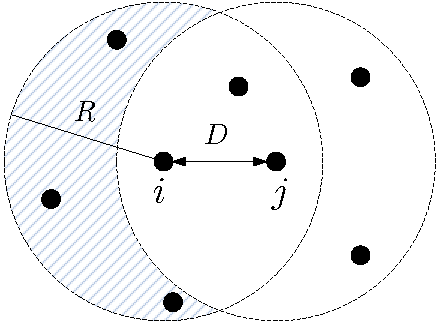
\includegraphics[width=5cm]{./model2.pdf}}
\caption{The network model}\label{fig:model2}
\end{figure}


 
\subsection{อัลกอริทึม II}
Add more subsections as you want.
\subsubsection{ขั้นตอนที่ 1}
\subsubsection{ขั้นตอนที่ 2}
Latex Format นี้รองรับหัวข้อย่อยถึงแค่ระดับ 4 นี้เท่านั้น ไม่แนะนำให้แบ่งหัวข้อย่อยไปมากกว่านี้ เช่น 2.2.2.2.1 , 2.2.2.2.2

\section{เครื่องมือที่ใช้ในการพัฒนา}

%%%%%%%%%%%%%%%%%%%%%%%%%%%%%%%%%%%%%%%%%%%%%%%%%%%%%55
%%%%%%%%%%%%%%%%%%%%%%%%%%%%%%%%%%%%%%%%%%%%%%%%%%%%%
%%%%%%%%%%%%%%%%%%%%%%%%%%%%%%%%%%%%%%%%%%%%%%%%%%%%%
\chapter{วิธีการดำเนินงาน}

\emph{หัวข้อต่าง ๆ ในแต่ละบทเป็นเพียงตัวอย่างเท่านั้น หัวข้อที่จะใส่ในแต่ละบทขึ้นอยู่กับโปรเจคของนักศึกษาและอาจารย์ที่ปรึกษา}


ตัวอย่างการใส่อ้างอิงที่มา -> \cite{hypersense} ถ้าต้องการใส่แหล่งอ้างอิงมากกว่า 1 ให้ทำดังนี้ -> \cite{hypersense,bworld} 
Explain the design (how you plan to implement your work) of your project. Adjust the section titles below to suit the types of your work. Detailed physical design like circuits and source codes should be placed in the appendix.

\section{ข้อกำหนดและความต้องการของระบบ}

\section{สถาปัตยกรรมระบบ}

\begin{table}[!h]
\centering
\caption{test table x1}\label{tbl:symbols}
\begin{tabular}{@{}p{0.07\textwidth}|p{0.7\textwidth}p{0.1\textwidth}}\hline
\multicolumn{2}{l}{\textbf{SYMBOL}}  & \textbf{UNIT} \\ \hline 
$\alpha$ & Test variable\hfill & m$^2$ \\
$\lambda$ & Interarrival rate\hfill &  jobs/second\\
$\mu$ & Service rate\hfill & jobs/second \\ \hline
\end{tabular}
%\begin{tabular}{c|c} \hline
% $\alpha$ & $\beta$ \\ \hline
% $\delta$ & $\mu$ \\ \hline
%\end{tabular}
\end{table}



\section{Hardware Module 1}
\subsection{Component 1}
\subsection{Logical Circuit Diagram}

\section{Hardware Module 2}
\subsection{Component 1}
\subsection{Component 2}

\section{Path Finding Algorithm}

\section{Database Design}

\section{UML Design}

\section{GUI Design}

\section{การออกแบบการทดลอง}
\subsection{ตัวชี้วัดและปัจจัยที่ศึกษา}
\subsection{รูปแบบการเก็บข้อมูล}




%%%%%%%%%%%%%%%%%%%%%%%%%%%%%%%%%%%%%%%%%%%%%%%%%%%%%%%%%%%%%%
%%%%%%%%%%%%%%%%%%%% Experiments %%%%%%%%%%%%%%%%%%%%%%%%%%%%%
%%%%%%%%%%%%%%%%%%%%%%%%%%%%%%%%%%%%%%%%%%%%%%%%%%%%%%%%%%%%%%%
\chapter{ผลการดำเนินงาน}


\emph{หัวข้อต่าง ๆ ในแต่ละบทเป็นเพียงตัวอย่างเท่านั้น หัวข้อที่จะใส่ในแต่ละบทขึ้นอยู่กับโปรเจคของนักศึกษาและอาจารย์ที่ปรึกษา}


ตัวอย่างการใส่อ้างอิงที่มา -> \cite{hypersense} ถ้าต้องการใส่แหล่งอ้างอิงมากกว่า 1 ให้ทำดังนี้ -> \cite{hypersense,bworld} 

You can title this chapter as \textbf{Preliminary Results} ผลการดำเนินงานเบื้องต้น or \textbf{Work Progress} ความก้าวหน้าโครงงาน for the progress reports. Present implementation or experimental results here and discuss them.
ใส่เฉพาะหัวข้อที่เกี่ยวข้องกับงานที่ทำ 

\section{ประสิทฺธิภาพการทำงานของระบบ} 
\section{ความพึงพอใจการใช้งาน}
\section{การวิเคราะห์ข้อมูลและผลการทดลอง}

%%%%%%%%%%%%%%%%%%%%%%%%%%%%%%%%%%%%%%%%%%%%%%%%%%%%%%%%%%%%%%%
%%%%%%%%%%%%%%%%%%%% Conclusions %%%%%%%%%%%%%%%%%%%%%%%%%%%%%
%%%%%%%%%%%%%%%%%%%%%%%%%%%%%%%%%%%%%%%%%%%%%%%%%%%%%%%%%%%%%%%
\chapter{บทสรุป}


\emph{หัวข้อต่าง ๆ ในแต่ละบทเป็นเพียงตัวอย่างเท่านั้น หัวข้อที่จะใส่ในแต่ละบทขึ้นอยู่กับโปรเจคของนักศึกษาและอาจารย์ที่ปรึกษา}



This chapter is optional for proposal and progress reports but 
is required for the final report.

\section{สรุปผลโครงงาน}
สรุปว่าโครงงานบรรลุตามวัตถุประสงค์ที่ตั้งไว้หรือไม่ อย่างไร 

\section{ปัญหาที่พบและการแก้ไข}
State your problems and how you fixed them.

\section{ข้อจำกัดและข้อเสนอแนะ}
ข้อจำกัดของโครงงาน What could be done in the future to make your projects better.

%%%%%%%%%%%%%%%%%%%%%%%%%%%%%%%%%%%%%%%%%%%%%%%%%%%%%%%%%%%%%%%
%%%%%%%%%%%%%%%%%%%% Bibliography %%%%%%%%%%%%%%%%%%%%%%%%%%%%%
%%%%%%%%%%%%%%%%%%%%%%%%%%%%%%%%%%%%%%%%%%%%%%%%%%%%%%%%%%%%%%%

%%%% Comment this in your report to show only references you have
%%%% cited. Otherwise, all the references below will be shown.
%\nocite{*}
%% Use the kmutt.bst for bibtex bibliography style 
%% You must have cpe.bib and string.bib in your current directory.
%% You may go to file .bbl to manually edit the bib items.

% Sept, 2021 by Thanin
% improve url breaks to prevent unnecessary big white spaces in some cases
\makeatletter
\g@addto@macro{\UrlBreaks}{\UrlOrds}
\makeatother
% 

\bibliographystyle{kmutt}
\bibliography{string,cpe}

%%%%%%%%%%%%%%%%%%%%%%%%%%%%%%%%%%%%%%%%%%%%%%%%%%%%%%%%%%%%%%%
%%%%%%%%%%%%%%%%%%%%%%%% Appendix %%%%%%%%%%%%%%%%%%%%%%%%%%%%%
%%%%%%%%%%%%%%%%%%%%%%%%%%%%%%%%%%%%%%%%%%%%%%%%%%%%%%%%%%%%%%%
\appendix{ชื่อภาคผนวกที่ 1}
\noindent{\large\bf ใส่หัวข้อตามความเหมาะสม} \\

This is where you put hardware circuit diagrams, detailed experimental data in tables or source codes, etc.. \\ \bigskip


 \begin{figure}[!h]
\caption{This is the figure x11 ทดสอบ จาก \href{https://www.google.com} {https://www.google.com}}\label{fig:x1}
\end{figure}


This appendix describes two static allocation methods for fGn (or fBm)
traffic. Here, $\lambda$ and $C$ are respectively the traffic arrival
rate and the service rate per dimensionless time step. Their unit are
converted to a physical time unit by multiplying the step size
$\Delta$. For a fBm self-similar traffic source,
Norros~\cite{norros95} provides its EB as
\begin{equation}\label{eq:norros}
  C = \lambda + (\kappa(H)\sqrt{-2\ln\epsilon})^{1/H}a^{1/(2H)}x^{-(1-H)/H}\lambda^{1/(2H)}
\end{equation}
where $\kappa(H) = H^H(1-H)^{(1-H)}$. Simplicity in the calculation is
the attractive feature of (\ref{eq:norros}).

The MVA technique developed in~\cite{kim01} so far provides the most
accurate estimation of the loss probability compared to previous
bandwidth allocation techniques according to simulation results.
Consider a discrete-time queueing system with constant service rate
$C$ and input process $\lambda_n$ with $\mathbb{E}\{\lambda_n\} =
\lambda$ and $\mathrm{Var}\{\lambda_n\} = \sigma^2$.  Define $X_n \equiv
\sum_{k=1}^n \lambda_k - Cn$.  The loss probability due to the MVA
approach is given by
\begin{equation}\label{eq:loss_mva}
  \varepsilon \approx \alpha e^{-m_x/2}
\end{equation}
where
\begin{equation}\label{eq:mx}
m_x = \min_{n \geq 0} \frac{((C-\lambda)n + B)^2}{\mathrm{Var}\{X_n\}} =
\frac{((C-\lambda)n^\ast + B)^2}{\mathrm{Var}\{X_{n^{\ast}}\}}
\end{equation} 
and 
\begin{equation}\label{eq:alpha}
  \alpha =
  \frac{1}{\lambda\sqrt{2\pi\sigma^2}}\exp\left(\frac{(C-\lambda)^2}{2\sigma^2}\right)
  \int_C^\infty (r-C)\exp\left(\frac{(r-\lambda)^2}{2\sigma^2}\right)\, dr
\end{equation}
For a given $\varepsilon$, we numerically solve for $C$ that satisfies
(\ref{eq:loss_mva}). Any search algorithm can be used to do the task.
Here, the bisection method is used.  

Next, we show how $\mathrm{Var}\{X_n\}$ can be determined.  Let
$C_{\lambda}(l)$ be the autocovariance function of $\lambda_n$.  The
MVA technique basically approximates the input process $\lambda_n$
with a Gaussian process, which allows $\mathrm{Var}\{X_n\}$ to be
represented by the autocovariance function.  In particular, the
variance of $X_n$ can be expressed in terms of $C_{\lambda}(l)$ as
\begin{equation}
  \mathrm{Var}\{X_n\} = nC_{\lambda}(0) + 2\sum_{l=1}^{n-1} (n-l)C_{\lambda}(l)
\end{equation} 
Therefore, $C_{\lambda}(l)$ must be known in the MVA technique, either
by assuming specific traffic models or by off-line analysis in case of
traces.  In most practical situations, $C_{\lambda}(l)$ will not be
known in advance, and an on-line measurement algorithm developed
in~\cite{eun01} is required to jointly determine both $n^\ast$ and
$m_x$. For fGn traffic, $\mathrm{Var}\{X_n\}$ is equal to $\sigma^2
n^{2H}$, where $\sigma^2 = \mathrm{Var}\{\lambda_n\}$, and we can find
the $n^\ast$ that minimizes (\ref{eq:mx}) directly. Although $\lambda$
can be easily measured, it is not the case for $\sigma^2$ and $H$.
Consequently, the MVA technique suffers from the need of prior
knowledge traffic parameters.


%%%%%%%%%%%%%%%%%%%%%%%%%%%%%%%%%%%%%%%%%%%%%%%%%%%%%%%%%%
%%%%%%%%%%%%%%% The 2nd appendix %%%%%%%%%%%%%%%%%%%%%%%%%%
%%%%%%%%%%%%%%%%%%%%%%%%%%%%%%%%%%%%%%%%%%%%%%%%%%%%%%%%%%
\appendix{ชื่อภาคผนวกที่ 2}
\noindent{\large\bf ใส่หัวข้อตามความเหมาะสม} \\


 \begin{figure}[!h]
\caption{This is the figure x11 ทดสอบ จาก \href{https://www.google.com} {https://www.google.com}}\label{fig:x1}
\end{figure}

Next, we show how $\mathrm{Var}\{X_n\}$ can be determined.  Let
$C_{\lambda}(l)$ be the autocovariance function of $\lambda_n$.  The
MVA technique basically approximates the input process $\lambda_n$
with a Gaussian process, which allows $\mathrm{Var}\{X_n\}$ to be
represented by the autocovariance function.  In particular, the
variance of $X_n$ can be expressed in terms of $C_{\lambda}(l)$ as
\begin{equation}
  \mathrm{Var}\{X_n\} = nC_{\lambda}(0) + 2\sum_{l=1}^{n-1} (n-l)C_{\lambda}(l)
\end{equation} 

\noindent{\large\bf Add more topic as you need} \\

Therefore, $C_{\lambda}(l)$ must be known in the MVA technique, either
by assuming specific traffic models or by off-line analysis in case of
traces.  In most practical situations, $C_{\lambda}(l)$ will not be
known in advance, and an on-line measurement algorithm developed
in~\cite{eun01} is required to jointly determine both $n^\ast$ and
$m_x$. For fGn traffic, $\mathrm{Var}\{X_n\}$ is equal to $\sigma^2
n^{2H}$, where $\sigma^2 = \mathrm{Var}\{\lambda_n\}$, and we can find
the $n^\ast$ that minimizes (\ref{eq:mx}) directly. Although $\lambda$
can be easily measured, it is not the case for $\sigma^2$ and $H$.
Consequently, the MVA technique suffers from the need of prior
knowledge traffic parameters. 





\end{document}
